\documentclass[12pt]{article}

\usepackage[utf8]{inputenc}
\usepackage[T1]{fontenc}
\usepackage{setspace}
\usepackage[margin=1in]{geometry}
\usepackage{amsmath,amssymb}
\usepackage{booktabs}
\usepackage{array}
\usepackage{graphicx}
\usepackage{natbib}
\usepackage{hyperref}
\usepackage{lmodern}
\usepackage{microtype}
\usepackage[format=plain,labelfont=bf,up,textfont=it,up]{caption}
\usepackage{float}

\hypersetup{
  colorlinks = true,
  linkcolor  = blue,
  citecolor  = blue,
  urlcolor   = blue
}

\doublespacing

\title{Election Forensics in a Polarized Democracy:\\
       Evidence from Peru's 2021 Presidential Runoff}

\author{Carlos C\'esar Ch\'avez Padilla%
  \thanks{Center for the Economics of Human Development,
          University of Chicago.
          Email: \href{mailto:cchavezp@uchicago.edu}{cchavezp@uchicago.edu}.
          I thank the Oficina Nacional de Procesos Electorales for making
          mesa-level data publicly available. All errors are my own.
          \textit{Data availability:} The primary data are publicly available
          at \url{https://datosabiertos.gob.pe}. Replication code is available
          at \url{https://github.com/cesarchavezp29/peru-election-forensics-2021}.}}

\date{March 2023}

% ─── convenience macros ───────────────────────────────────────────────────────
\newcommand{\pct}[1]{#1\,\%}
\newcommand{\N}[1]{\num{#1}}
\usepackage{siunitx}
\sisetup{group-separator={,}, group-minimum-digits=4}

% ─────────────────────────────────────────────────────────────────────────────
\begin{document}

\maketitle
\thispagestyle{empty}

% ─── Abstract ────────────────────────────────────────────────────────────────
\begin{abstract}
\noindent
Peru's 2021 presidential runoff between Pedro Castillo and Keiko Fujimori
produced the closest result in modern Peruvian history---a margin of 44,263
votes out of 17 million cast. Fujimori refused to concede, alleged systematic
fraud, and delayed certification by six weeks. I apply multiple forensic
methods to the complete universe of polling-station records published by
Peru's electoral authority (ONPE): distributional fingerprint analysis
\citep{klimek2012}, last-digit uniformity tests \citep{beber2012}, and
ecological regression comparing first- and second-round results. I also
exploit the institutional distinction between \emph{contested} actas---those
resolved by the electoral tribunal after challenge---and uncontested actas as
a within-election test. No method detects patterns consistent with vote
manipulation. Contested and uncontested polling stations show identical
forensic signatures once geographic location is taken into account. The data
instead reveal extreme geographic polarization: Castillo received over 80\,\%
of valid votes in southern highland departments while Fujimori dominated coastal
and metropolitan areas. These findings contribute to the election forensics
literature and illustrate how geographic polarization can generate vote
distributions that appear anomalous to non-specialists, fueling fraud
narratives even in clean elections.

\medskip
\noindent\textbf{Keywords:} election forensics, electoral fraud, Peru,
geographic polarization, distributional fingerprints, digit tests.

\medskip
\noindent\textbf{JEL codes:} D72, C12, P16.
\end{abstract}

\newpage

% =============================================================================
\section{Introduction}
\label{sec:intro}
% =============================================================================

On June 6, 2021, Peruvians cast ballots in a presidential runoff between
Pedro Castillo of Peru Libre and Keiko Fujimori of Fuerza Popular. When the
final count closed, Castillo had won by 44,263 votes---50.13\,\% to 49.87\,\%
of valid votes, a margin of 0.26 percentage points. It was the narrowest
presidential result in modern Peruvian history.

Fujimori did not concede. Hours after voting ended, she held a press
conference alleging ``systematic fraud'' in rural polling stations. Her legal
team filed nullification challenges (\emph{solicitudes de nulidad}) against
over 800 individual \emph{actas} (polling-station tally sheets), primarily in
highland and Amazonian departments. The \emph{Jurado Nacional de Elecciones}
(JNE)---Peru's electoral court---reviewed each challenge, rejected most, and
certified the result on July 19, six weeks after election day. The
Organization of American States and the European Union electoral observation
missions both reported finding no evidence of systematic irregularities
\citep{oas2021, eu2021}. Fujimori's supporters organized street protests
through much of July. The fraud narrative did not dissipate; it persisted
throughout Castillo's turbulent presidency and was still circulating after his
removal from office in December 2022.

This paper provides the first comprehensive forensic analysis of Peru 2021
at the polling-station level. I use the complete universe of 82,870 domestic
\emph{mesas} (polling stations) in the ONPE data, applying four independent
methods: distributional fingerprint plots \citep{klimek2012}, last-digit
uniformity tests \citep{beber2012}, ecological regression linking first- and
second-round vote shares, and geographic mapping of null-vote rates. I also
exploit a feature of the Peruvian counting process that has not been used in
prior forensic studies: the distinction between \emph{contabilizada} actas
(tallied without challenge) and \emph{computada resuelta} actas (challenged
and resolved by the JNE tribunal). If fraud occurred specifically in the
contested subset---which is the direct implication of Fujimori's allegations---
the two groups should differ on forensic diagnostics. They do not.

The central finding is that no method detects statistical anomalies consistent
with manipulation. Turnout never exceeds 100\,\% at any polling station.
Last-digit distributions pass chi-squared uniformity tests in all four
candidate-by-status groups, with $p$-values ranging from 0.19 to 0.91.
The ecological regression shows that districts with higher concentrations of
contested actas do not over-perform for Castillo relative to their first-round
baseline: the interaction coefficient is positive but statistically
insignificant ($p = 0.71$). The dominant pattern is extreme geographic
sorting---Castillo's vote share exceeded 80\,\% in many southern highland
provinces and fell below 35\,\% in Lima---which is consistent with Peru's
deep economic and cultural divide between the \emph{costa} and the
\emph{sierra}.

The paper relates to a growing literature on quantitative election forensics.
\citet{klimek2012} develop the distributional fingerprint method using Russian
and Austrian data. \citet{beber2012} formalize the last-digit test and apply
it to African elections. \citet{myagkov2009} study Russian and Ukrainian
elections using a range of ecological methods. \citet{kobak2016} document
integer-percentage clustering in Russian results. The Latin American context
has received less attention, though the 2019 Bolivian election generated a
substantial methodological debate: \citet{idrobo2022} show that the shift
toward Morales in the late count was consistent with normal differential
reporting speeds and did not require fraud as an explanation, while
\citet{escobari2024} argue that the discontinuity in vote transmission was
real and indicative of manipulation. Peru 2021 differs from Bolivia 2019 in a
structural way---there was no halt or disruption in the ONPE counting
process---but both cases illustrate how geographic polarization and
differential reporting speeds can make legitimate elections appear suspicious.

The only prior forensic analysis of Peru 2021 is \citet{isea2021}, who apply
Benford's law to department-level aggregates and find no fraud signature. The
present paper improves on that analysis in three ways: it uses mesa-level data
(more than 80,000 observations versus 25 departments), it applies multiple
methods with different identifying assumptions, and it introduces the
contested/uncontested comparison as a direct test of the specific claims made
by Fujimori's legal team.

Close elections generating fraud allegations that undermine democratic
legitimacy have become a recurring pattern. \citet{eggers2021} provide a
comprehensive forensic examination of claims about the 2020 U.S. election and
find no evidence supporting them. Similar dynamics have unfolded in multiple
elections across Latin America and beyond \citep{lehoucq2003, hyde2007}.
Statistical analysis provides the evidentiary baseline against which other
claims must be weighed.

The data and methods are described in Sections~\ref{sec:data} and
\ref{sec:methods}. Results follow in Section~\ref{sec:results}, with a
discussion of mechanisms and limitations in Section~\ref{sec:discussion}.

% =============================================================================
\section{The 2021 Peruvian Presidential Election}
\label{sec:background}
% =============================================================================

\subsection{First round}

The first round was held on April 11, 2021, with 18 candidates. Fragmentation
was extreme: no candidate crossed 20\,\% of valid votes. Castillo of Peru
Libre finished first with 19.1\,\%, a narrow margin above Fujimori's 13.4\,\%
(Fuerza Popular). The remaining 67\,\% of the vote was split among 16 other
candidates, many representing centrist or right-of-center positions. Candidates
who might have been expected to coalesce voters against both Castillo and
Fujimori---Hernando de Soto, Yonhy Lescano, Rafael L\'opez Aliaga---each
obtained between 8\,\% and 12\,\%, preventing any single moderate from
advancing to the runoff. The outcome was shaped by Peru's fragmented party
system, which \citet{mainwaring2018} and others have documented as one of the
most weakly institutionalized in Latin America.

\subsection{Runoff dynamics}

The runoff produced binary consolidation along geographic and class lines.
Castillo drew on deep opposition to the Fujimori family---Keiko's father,
Alberto Fujimori, governed as an authoritarian from 1990 to 2000 and was
serving a prison sentence for human rights violations and corruption during the
election---and on genuine enthusiasm in the rural highlands for his program of
resource nationalism and constitutional reform. Fujimori consolidated urban,
coastal, and upper-middle-class voters behind an anti-communist, anti-Castillo
message.

Geographic polarization intensified sharply from the first round to the
runoff. Southern highland departments that had given Castillo 25--35\,\% in
April delivered 80--90\,\% in June. Coastal departments that had split among
many candidates moved to Fujimori at 55--65\,\%. Peru Libre's 19\,\% first-round
national share nearly tripled in the second round, while Fuerza Popular's
13\,\% roughly quadrupled---both reflecting the binary-choice effect of a
two-candidate contest in a deeply polarized electorate.

\subsection{The fraud allegations}

Exit polls and early partial counts on June 6 showed a very close race with
Fujimori holding a narrow lead from faster-reporting coastal precincts. As
highland results arrived over the following days, Castillo's total grew. On
June 9, with roughly 80\,\% of actas counted, Castillo took the lead and never
relinquished it. Fujimori's campaign attributed the shift to fraud, arguing
that highland tallies had been systematically altered.

Her legal team filed nullification challenges against 802 individual actas
across multiple departments. The challenges alleged procedural violations:
unsigned tally sheets, incorrect vote totals, absent party observers. The JNE
processed each challenge individually over a six-week period. The vast majority
were rejected. A subset of challenged actas was reclassified as
\emph{computada resuelta} after JNE review and incorporated into the final
count. Certification was issued on July 19, 2021 \citep{jne2021}.
International observers from the OAS and EU found no evidence of systematic
irregularities in either the voting or the counting process \citep{oas2021,
eu2021}.

\subsection{Political aftermath}

Castillo took office on July 28, 2021. His government was marked by
instability: he cycled through four prime ministers in his first year and faced
repeated congressional attempts at removal through a constitutional mechanism
permitting impeachment for ``moral incapacity.'' Two such attempts failed. On
December 7, 2022, Castillo attempted to dissolve Congress by decree---a step
with no constitutional basis---and announced a curfew. The JNE declared his
action unconstitutional. Congress voted to remove him, and he was arrested the
same day. Vice President Dina Boluarte assumed the presidency. Throughout this
period, segments of the population continued to believe the 2021 election had
been stolen, illustrating the durable damage that sustained fraud allegations
can inflict on democratic legitimacy even after courts have adjudicated them.

% =============================================================================
\section{Data}
\label{sec:data}
% =============================================================================

\subsection{Source and structure}

The primary data source is the ONPE open data portal
(\url{https://datosabiertos.gob.pe}), which published the complete mesa-level
results as a semicolon-delimited file with 86,488 rows, one per polling station
\citep{onpe2021}. Each row contains the polling station identifier
(\texttt{MESA\_DE\_VOTACION}), a six-digit location code (\texttt{UBIGEO}),
geographic labels (department, province, district), a status variable
(\texttt{DESCRIP\_ESTADO\_ACTA}), registered voters (\texttt{N\_ELEC\_HABIL}),
total votes cast (\texttt{N\_CVAS}), votes for Castillo/Peru Libre
(\texttt{VOTOS\_P1}), votes for Fujimori/Fuerza Popular (\texttt{VOTOS\_P2}),
null votes (\texttt{VOTOS\_VN}), blank votes (\texttt{VOTOS\_VB}), and
challenged/impugned votes (\texttt{VOTOS\_VI}).

\subsection{Sample construction}

The status variable takes five values. I keep \texttt{CONTABILIZADA}
(fully counted, 84,863 polling stations) and \texttt{COMPUTADA RESUELTA}
(challenged and resolved by JNE, 1,386 polling stations). I drop
\texttt{ANULADA} (annulled, 213), \texttt{EN PROCESO} (in process, 20), and
\texttt{SIN INSTALAR} (not installed, 6). The final-status sample of
86,249 mesas covers all polling stations for which the count is definitively
closed.

I exclude overseas polling stations, which report under five continental
jurisdiction labels (Am\'erica, Europa, Asia, Ocean\'ia, and \'Africa).
Overseas mesas differ structurally from domestic ones: turnout averaged
36.2\,\% overseas versus 76.1\,\% domestically, and the overseas electorate
favored Fujimori by 66.2\,\% to 33.8\,\%---reflecting the demographic
composition of the Peruvian diaspora. Including overseas results would confound
the geographic patterns that are central to the forensic analysis. I report
overseas totals separately in Table~\ref{tab:summary}.

The domestic analysis sample comprises 82,870 polling stations: 81,793
\emph{contabilizada} (uncontested) and 1,077 \emph{computada resuelta}
(contested).

\subsection{Key variables}

Turnout is defined as total votes cast divided by registered voters. Castillo
share is Castillo votes divided by valid votes (Castillo plus Fujimori). Valid
votes exclude null and blank ballots. The contested indicator equals one for
\emph{computada resuelta} polling stations and zero for \emph{contabilizada}
stations. For the digit tests, I extract the last digit of each candidate's
vote count at the polling station level.

\subsection{Complementary data}

First-round results come from the same ONPE portal \citep{onpe2021a}, with the
same status filter applied. Castillo (Peru Libre) is identified as candidate
16 (\texttt{VOTOS\_P16}) in the first-round file, verified by matching the
national aggregate to the official published figure of approximately 19.1\,\%.
My calculation yields 19.06\,\% for the domestic final-status sample, consistent
with official totals. District-level merging between rounds uses the
\texttt{UBIGEO} six-digit code as the join key. For province-level mapping I
use GADM 4.1 shapefiles, matching on normalized (accent-stripped, punctuation-removed)
department and province name pairs; 193 of 195 GADM provinces match, with the two
remaining unmatched being a structural GADM artifact (Lima province listed under
a separate administrative level) and a water-body polygon (Lago Titicaca) with
no assigned voters.

\begin{table}[H]
\caption{National Summary Statistics, Peru 2021 Presidential Runoff}
\label{tab:summary}
\medskip
\small
\begin{tabular}{lrr}
\toprule
 & \textbf{Domestic} & \textbf{Overseas} \\
 & (main analysis) & (separate) \\
\midrule
Polling stations (mesas) & 82,870 & 3,379 \\
\quad Uncontested (\emph{contabilizada}) & 81,793 & --- \\
\quad Contested (\emph{computada resuelta}) & 1,077 & --- \\
Registered voters & 24,238,529 & 980,061 \\
Votes cast & 18,454,387 & 354,330 \\
Turnout & 76.14\,\% & 36.15\,\% \\
\midrule
Valid votes & 17,291,272 & 333,259 \\
Castillo (VOTOS\_P1) & 8,721,769 & 112,671 \\
\quad Share of valid votes & 50.44\,\% & 33.81\,\% \\
Fujimori (VOTOS\_P2) & 8,569,503 & 220,588 \\
\quad Share of valid votes & 49.56\,\% & 66.19\,\% \\
Net margin (Castillo $-$ Fujimori) & $+$152,266 & $-$107,917 \\
\midrule
Null votes & 1,043,651 & 19,073 \\
\quad Share of votes cast & 5.66\,\% & 5.38\,\% \\
Blank votes & 119,464 & 1,998 \\
\quad Share of votes cast & 0.65\,\% & 0.56\,\% \\
\bottomrule
\end{tabular}
\medskip

\small\textit{Notes:}
The domestic sample comprises all polling stations with final status
CONTABILIZADA or COMPUTADA RESUELTA, excluding overseas jurisdictions
(Am\'erica, Europa, Asia, Ocean\'ia, \'Africa).
The all-rows Castillo$-$Fujimori margin is 44,240, within 23 votes
of the official JNE-certified margin of 44,263; the trivial discrepancy
arises from rounding in dropped rows (ANULADA and EN PROCESO).
\textit{Source:} ONPE, Resultados por mesa de las Elecciones Presidenciales
2021 Segunda Vuelta \citep{onpe2021}.
\end{table}

The domestic margin of $+152{,}266$ reflects Castillo's dominant performance
in the sierra and selva regions. The overseas margin of $-107{,}917$ reflects
the Lima-centric composition of the Peruvian diaspora, which voted heavily
for Fujimori at a turnout rate less than half the domestic average.
Together they reconcile to the official certified margin of 44,263.

\begin{table}[H]
\caption{Anomaly Flags: Distributional Extremes in the Domestic Final-Status Sample}
\label{tab:flags}
\medskip
\small
\begin{tabular}{lrr}
\toprule
Anomaly criterion & Mesas flagged & \% of sample \\
\midrule
Turnout $> 100\,\%$ & 0 & 0.00 \\
Turnout $< 10\,\%$ (and registered voters $> 0$) & 2 & 0.00 \\
Null vote rate $> 30\,\%$ of cast & 319 & 0.39 \\
Castillo share $= 100\,\%$ (and valid votes $\geq 10$) & 70 & 0.08 \\
Fujimori share $= 100\,\%$ (and valid votes $\geq 10$) & 3 & 0.00 \\
Turnout $> 98\,\%$ & 57 & 0.07 \\
\bottomrule
\end{tabular}
\medskip

\small\textit{Notes:}
Flags computed on the domestic final-status sample of 82,870 mesas.
The 70 mesas with 100\,\% Castillo share are concentrated in rural highland
districts (Puno, Ayacucho, Apur\'imac) where genuine near-unanimity is
historically documented. The 57 very-high-turnout mesas do not cluster in
any particular region. Zero mesas exceed 100\,\% turnout.
\textit{Source:} ONPE \citep{onpe2021}; author's calculations.
\end{table}

The anomaly flag counts reveal no systematic indicators of fraud. The 319 mesas
with high null rates deserve further inspection: as Figure~\ref{fig:map_nullvotes}
shows, they are concentrated in coastal departments rather than in Castillo's
highland strongholds, consistent with protest voting rather than targeted
invalidation of pro-Castillo ballots.

% =============================================================================
\section{Methods}
\label{sec:methods}
% =============================================================================

\subsection{Distributional fingerprint analysis}

\citet{klimek2012} introduced the distributional fingerprint method after
applying it to Russian and Austrian elections. The method plots polling-station
turnout on the horizontal axis against the winner's vote share on the vertical
axis. Under genuine counting, the resulting scatter forms a dispersed cloud
with no strong correlation structure: turnout and vote share vary
independently across precincts, with both driven primarily by local demographic
conditions. Two forms of manipulation produce characteristic departures from
this pattern. Ballot stuffing---fabricating votes for one candidate and
reporting them as if cast---inflates both turnout and the winner's share
simultaneously, extending the cloud toward the upper-right corner
(high turnout, high winner share) in a finger-like protrusion. Vote
stealing---switching cast votes from one candidate to the other---shifts the
cloud rightward (higher winner share) without increasing turnout.

A critical limitation of this approach in polarized elections is that genuine
regional clusters can produce a pattern that mimics ballot stuffing. If one
region has both high political loyalty to a candidate and high mobilization
capacity, it will occupy the upper-right of the scatter even in a clean
election. Peru's southern highlands are precisely such a region. To address
this, I color observations by macro-region (Costa, Sierra, Selva) and verify
that the regional structure accounts for any clustering before drawing
forensic conclusions.

I additionally superimpose contested mesas (COMPUTADA RESUELTA) on the same
plot as orange dots. If the fraud allegations are correct---if those specific
polling stations were where manipulation occurred---they should cluster
disproportionately in the upper-right corner. Observing that they scatter
throughout the same cloud as uncontested mesas would be inconsistent with
the fraud hypothesis.

\subsection{Last-digit uniformity tests}

\citet{beber2012} establish the statistical basis for digit-based fraud
detection. When vote totals are genuinely counted, the last digit of each
count should be approximately uniformly distributed across 0--9, since the
last digit carries no information that round-number selection could exploit.
When humans fabricate or alter vote counts, they tend to choose round numbers
(ending in 0 or 5), producing detectable heaping. The test statistic is the
standard chi-squared goodness-of-fit test against a uniform distribution over
10 categories, with $9$ degrees of freedom.

This test is more appropriate for Peruvian mesa-level data than Benford's
law, which requires vote counts to span multiple orders of magnitude
\citep{deckert2011}. With Peruvian mesas typically registering around 200
registered voters, the count distributions are narrow and Benford's law does
not apply. \citet{isea2021} apply Benford tests to department-level
aggregates for Peru 2021; the present analysis uses the more
powerful mesa-level digit test.

I run the test separately for four groups: (1) Castillo votes at uncontested
mesas, (2) Castillo votes at contested mesas, (3) Fujimori votes at
uncontested mesas, and (4) Fujimori votes at contested mesas. The four-way
breakdown is the paper's primary test of the fraud allegations. If vote totals
in contested actas were altered, the last-digit distribution in groups 2 or 4
should depart from uniformity relative to groups 1 or 3. I exclude zeros
from each test because mesas with zero votes for a candidate have no last
digit in the usual sense.

\subsection{Ecological regression}

At the district level (Peru has approximately 1,900 districts), I aggregate
polling-station results to compute Castillo's second-round vote share and
Peru Libre's first-round vote share. The regression is:

\begin{equation}
  \text{share}_{2v,d} = \alpha + \beta_1 \, \text{share}_{1v,d} + \varepsilon_d
  \label{eq:spec1}
\end{equation}

where $\text{share}_{2v,d}$ is Castillo's valid-vote share in district $d$ in
the segunda vuelta and $\text{share}_{1v,d}$ is Peru Libre's valid-vote share
in the first round. The first round featured 18 candidates, so Peru Libre's
share was compressed near 19\,\% nationally; the runoff forced a binary choice
and mechanically expanded both candidates' shares. The slope $\beta_1$ captures
the persistence of geographic preferences across rounds. An intercept near
0.40 is expected: in districts where Peru Libre got zero votes in the first
round, Castillo would still attract \emph{anti-Fujimori} votes from former
supporters of other first-round candidates.

I extend this with a second specification that adds the district-level share
of contested mesas and its interaction with first-round share:

\begin{equation}
  \text{share}_{2v,d} = \alpha + \beta_1 \, \text{share}_{1v,d}
    + \gamma \, \text{share\_cont}_d
    + \delta \, (\text{share}_{1v,d} \times \text{share\_cont}_d)
    + \varepsilon_d
  \label{eq:spec2}
\end{equation}

The coefficient $\gamma$ captures any level shift in Castillo's second-round
share associated with a higher concentration of contested mesas, after
controlling for first-round baseline. The interaction coefficient $\delta$
tests whether the relationship between first- and second-round shares changes
in districts with more contested mesas. A positive $\gamma$ or positive
$\delta$ would be consistent with manipulation in contested areas
(Castillo over-performing in proportion to the share of challenged actas).
A negative $\gamma$ would be consistent with the institutional reality that
contested actas are concentrated in Fujimori territory. Standard errors are
HC0-robust throughout.

\subsection{Null vote geography}

Null votes are ballots cast that were not counted as valid (typically because
the voter marked multiple candidates, left the ballot blank in the wrong way,
or otherwise spoiled it). If fraud took the form of systematic invalidation of
pro-Castillo votes, null rates should be elevated in highland departments where
Castillo received high vote shares. If null votes reflect protest behavior by
voters who disliked both candidates, they should concentrate in areas with
neither strong Castillo nor strong Fujimori support. I map null vote rates at
the province level and inspect the geographic pattern.

\subsection{What these tests cannot detect}

Forensic methods detect statistical signatures consistent with specific types of
manipulation. They do not prove the absence of fraud. A manipulation that
perfectly mimics the statistical properties of genuine counting would be
undetectable by any of these methods. The appropriate claim is the more modest
one: the data are consistent with a clean count, and inconsistent with the
specific forms of manipulation alleged by Fujimori's legal team (alteration of
recorded vote totals in specific actas).

The strongest available test for vote-count manipulation---regression
discontinuity analysis of the counting sequence, as employed by
\citet{escobari2024} for Bolivia---cannot be implemented for Peru 2021. ONPE
did not publish mesa-level processing timestamps with the results data. I
attempted to reconstruct a counting sequence from a GitHub repository of
scraped ONPE data; the timestamps in that dataset were uniform (a single bulk
download), providing no counting-order information. If ONPE were to release
internal processing logs, the temporal test could be implemented.

These tests address the specific fraud allegations: that recorded vote totals
in already-cast actas were altered. They do not address pre-electoral
irregularities such as voter intimidation, vote buying, or registration fraud,
which require different data.

% =============================================================================
\section{Results}
\label{sec:results}
% =============================================================================

\subsection{Geographic patterns}

Peru 2021 was among the most geographically polarized elections in recent Latin
American history. Table~\ref{tab:summary} shows the domestic aggregate: Castillo
won 50.44\,\% of valid votes, Fujimori 49.56\,\%, on a national turnout of
76.1\,\% among 24.2 million registered domestic voters. These national averages
conceal massive regional variation.

\begin{figure}[H]
\centering
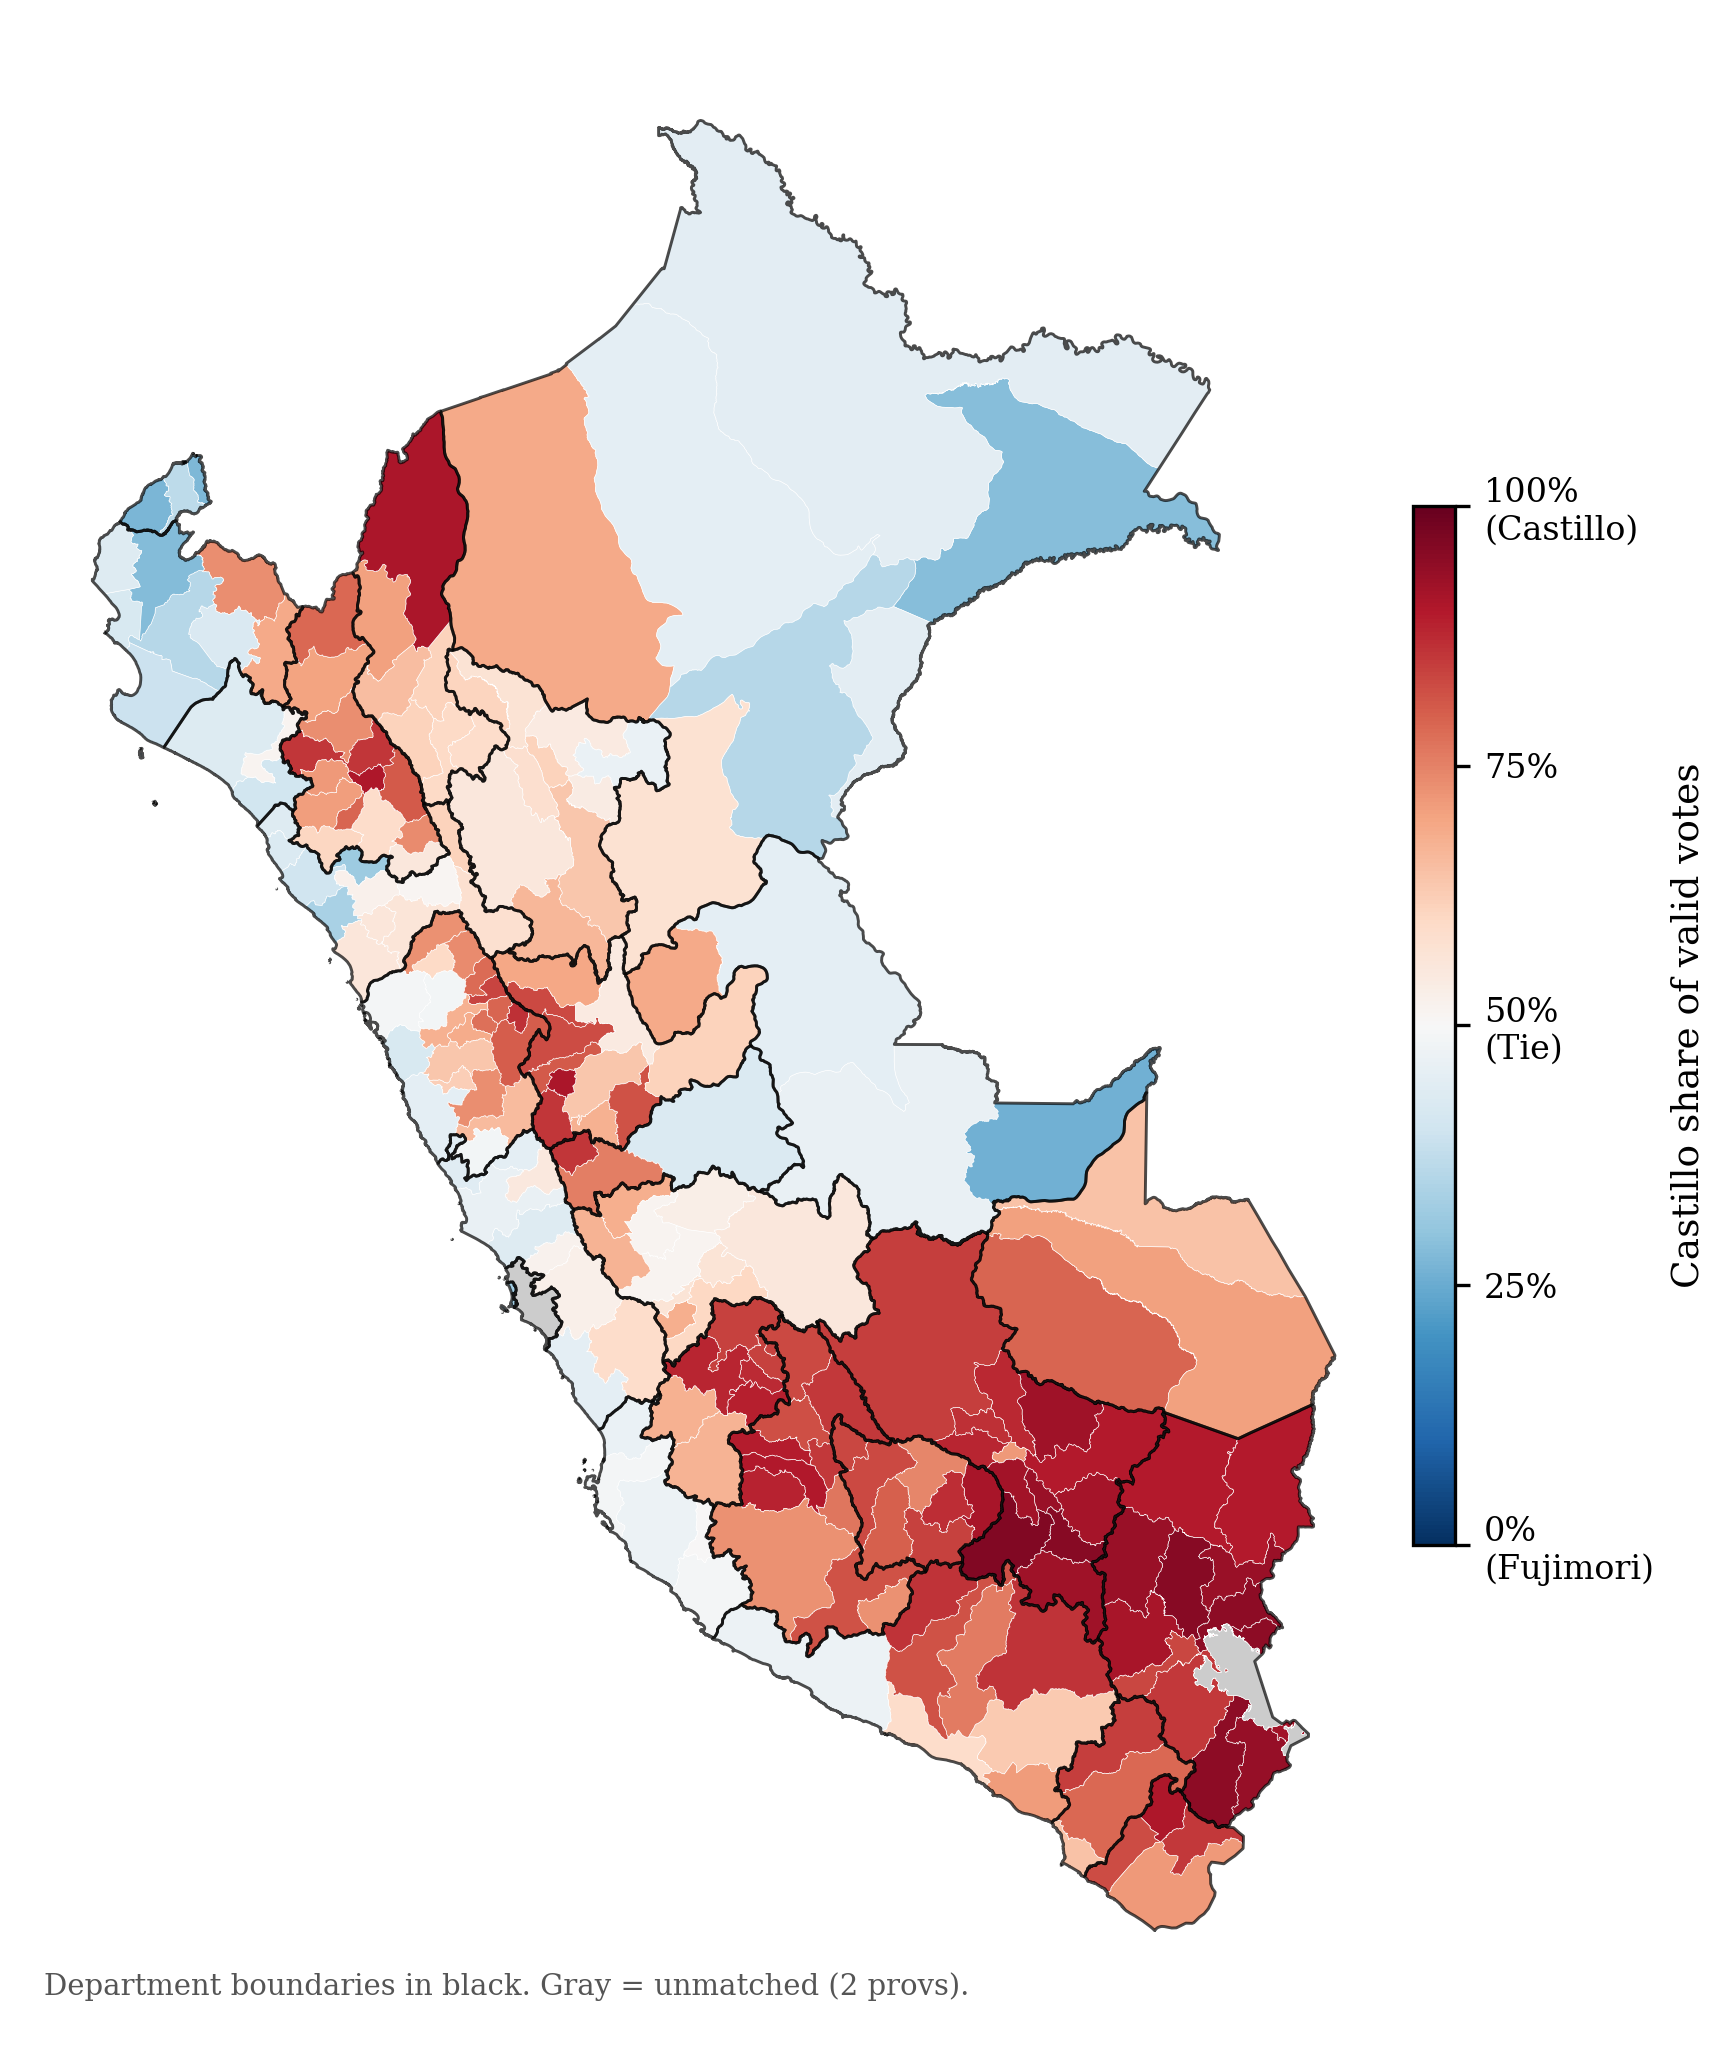
\includegraphics[width=0.88\textwidth]{fig1_map_castillo.png}
\caption{Castillo vote share by province, segunda vuelta 2021.
         Colors run from dark blue (Fujimori strongholds, share near 0)
         to dark red (Castillo strongholds, share near 1).
         The geographic polarization between the Andean highlands and
         the Pacific coast is the dominant feature of the data.}
\label{fig:map_castillo}
\medskip
\small\textit{Note:} Province-level aggregates from the domestic final-status
sample (82,870 mesas). Two GADM polygons (Lima Province administrative
boundary and Lago Titicaca) are not matched to ONPE data and appear grey.
\textit{Source:} ONPE \citep{onpe2021}; GADM 4.1 shapefiles; author's calculations.
\end{figure}

Figure~\ref{fig:map_castillo} maps Castillo's vote share by province. The
geographic pattern is stark. Puno gave Castillo 89.3\,\% of valid votes.
Huancavelica delivered 84.8\,\%, Cusco 83.2\,\%, Ayacucho 82.6\,\%, and
Apur\'imac 81.5\,\%. At the other extreme, Lima voted 64.6\,\% for Fujimori
and Callao 67.4\,\%. The map shows a near-continuous highland bloc
stretching from Puno in the south through the central sierra to Cajamarca and
Amazonas in the north, all voting 60--90\,\% for Castillo, ringed by coastal
departments where Fujimori dominated.

\begin{figure}[H]
\centering
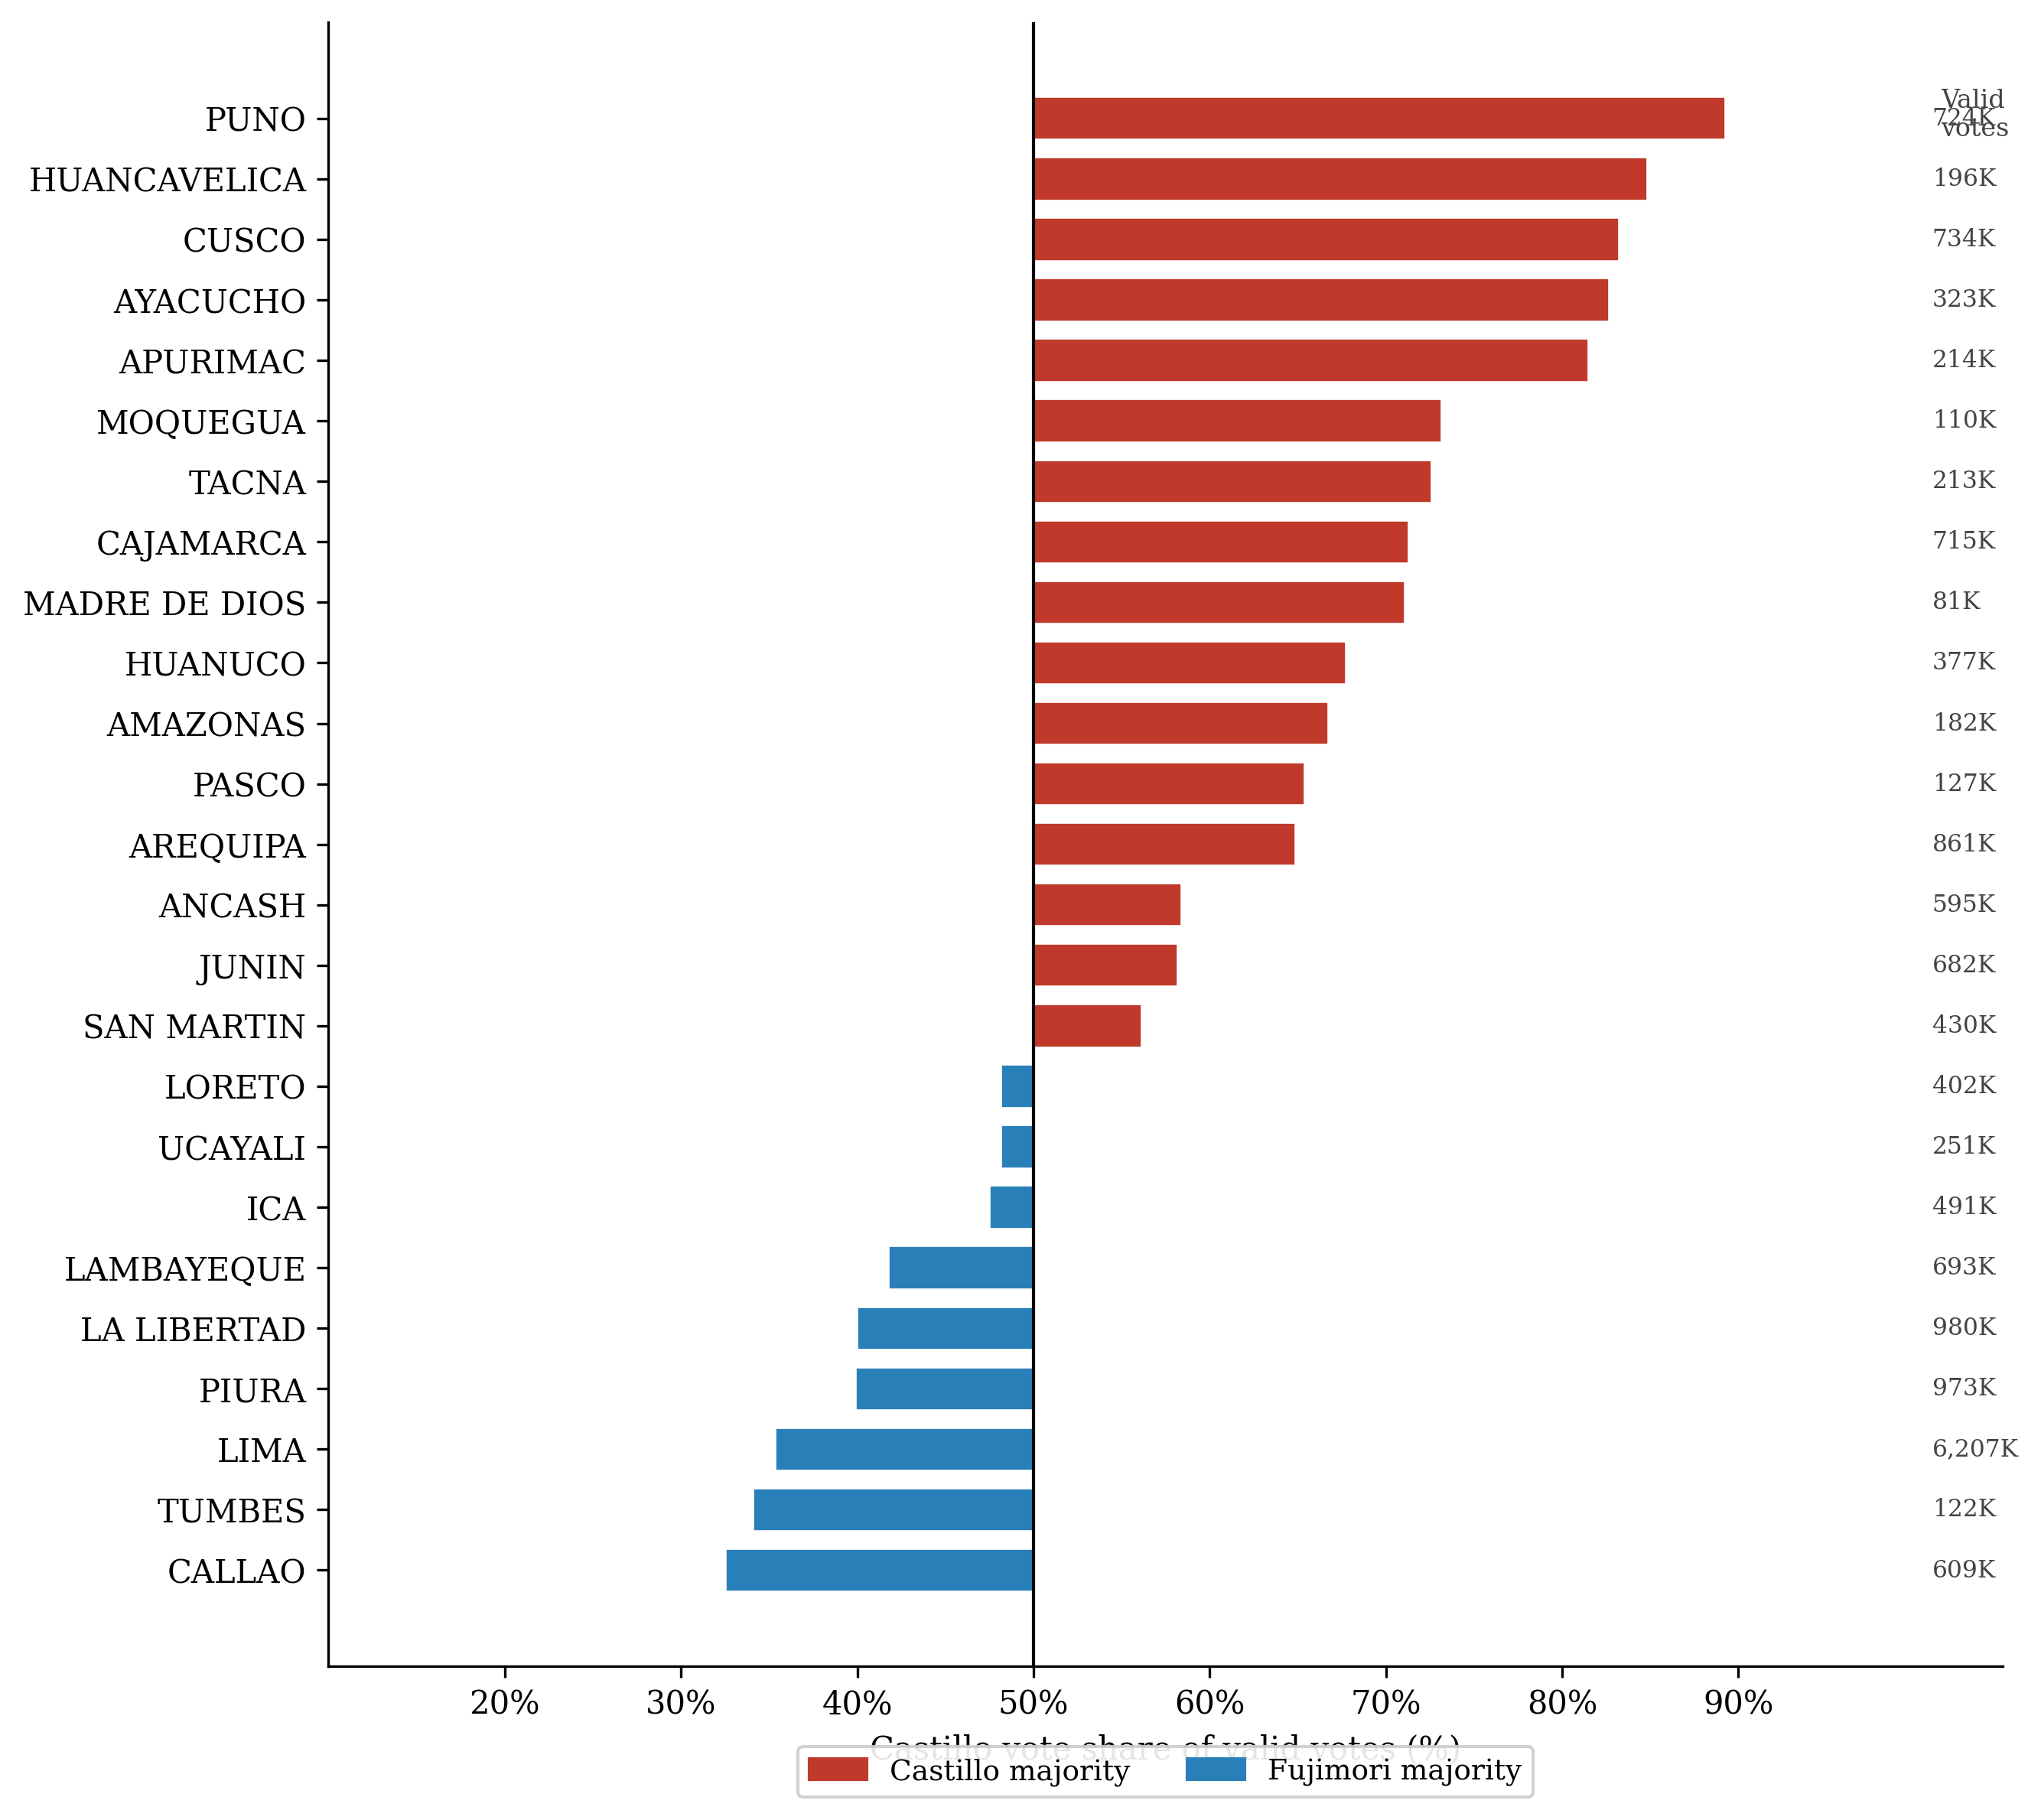
\includegraphics[width=0.90\textwidth]{fig6_dept_bars.png}
\caption{Castillo valid-vote share by department, segunda vuelta 2021.
         Departments sorted by Castillo share ascending.
         Horizontal line at 50.44\,\% marks the national domestic average.}
\label{fig:dept_bars}
\medskip
\small\textit{Note:} Department-level aggregates from the domestic
final-status sample. The range runs from below 35\,\% (Lima, Callao, Tacna)
to above 89\,\% (Puno).
\textit{Source:} ONPE \citep{onpe2021}; author's calculations.
\end{figure}

Figure~\ref{fig:dept_bars} shows Castillo's valid-vote share by department.
No highland department gave Castillo less than 55\,\% of valid votes.
No coastal department gave him more than 50\,\%. This geographic sorting is
the baseline against which all forensic results must be interpreted: any
pattern that correlates with geography in this election is more likely
explained by genuine political preferences than by manipulation.

\subsection{The contested actas}

The paper's distinctive test exploits the institutional record of the JNE
challenge process. Table~\ref{tab:contested} reports the comparison.

\begin{table}[H]
\caption{Contested vs.\ Uncontested Polling Stations}
\label{tab:contested}
\medskip
\small
Panel A: Vote totals and shares
\medskip

\begin{tabular}{lrrr}
\toprule
 & Uncontested & Contested & Total \\
 & (CONTABILIZADA) & (COMP.\ RESUELTA) & \\
\midrule
Mesas & 81,793 & 1,077 & 82,870 \\
Total Castillo votes & 8,628,619 & 93,150 & 8,721,769 \\
Total Fujimori votes & 8,437,103 & 132,400 & 8,569,503 \\
Net margin (C$-$F) & $+$191,516 & $-$39,250 & $+$152,266 \\
\midrule
Avg.\ turnout & 76.13\,\% & 76.43\,\% & 76.14\,\% \\
Avg.\ Castillo share & 51.42\,\% & 42.11\,\% & 51.30\,\% \\
Avg.\ Fujimori share & 48.58\,\% & 57.89\,\% & 48.70\,\% \\
Avg.\ null rate & 5.62\,\% & 7.08\,\% & 5.64\,\% \\
\bottomrule
\end{tabular}

\medskip
Panel B: Geographic distribution of contested mesas
\medskip

\begin{tabular}{lrrr}
\toprule
Macro-region & Contested mesas & Total mesas & Contestation rate \\
\midrule
Costa & 848 & 54,900 & 1.54\,\% \\
Selva & 118 & 9,424 & 1.25\,\% \\
Sierra & 111 & 18,546 & 0.60\,\% \\
\midrule
\textbf{Total} & \textbf{1,077} & \textbf{82,870} & \textbf{1.30\,\%} \\
\bottomrule
\end{tabular}
\medskip

\small\textit{Notes:}
Average shares are unweighted means across polling stations.
Costa includes Lima, La Libertad, Lambayeque, Piura, Ica,
Arequipa, Moquegua, Tacna, Tumbes, \'Ancash, and Lima Provincias.
\'Ancash spans both coastal and highland provinces; I assign it to Costa
following INEI's conventional macro-regional classification.
Reassigning \'Ancash to Sierra does not change any result.
Sierra is the remaining highland departments; Selva the Amazonian departments.
Challenged actas are concentrated in Fujimori's stronghold (Costa, and Lima
in particular) rather than in Castillo's highland support base.
\textit{Source:} ONPE \citep{onpe2021}; JNE \citep{jne2021}; author's calculations.
\end{table}

Of 82,870 domestic final-status polling stations, 1,077 (1.30\,\%) are
\emph{computada resuelta}---contested and resolved. These mesas break
42.1\,\% Castillo / 57.9\,\% Fujimori, compared with 51.4\,\% / 48.6\,\% in
the 81,793 uncontested stations. The contested mesas net out to a Fujimori
advantage of 39,250 votes; the uncontested mesas net a Castillo advantage of
191,516. The domestic net is $+152{,}266$ for Castillo; combined with the
$-107{,}917$ overseas margin (where Fujimori dominated 66.2\,\% to 33.8\,\%),
the all-rows margin is 44,240---within 23 votes of the official 44,263.

The geographic distribution of contested mesas, shown in
Figure~\ref{fig:map_contested}, runs directly against the fraud hypothesis.
Lima accounts for 555 of 1,077 domestic contested mesas (51.5\,\%). The
contestation rate is 1.99\,\% in Lima, 1.71\,\% in Callao, and 1.54\,\%
across all Costa departments---compared with 1.25\,\% in the Selva and
0.60\,\% in the Sierra. Challenges were concentrated in Fujimori's own
territory, not in Castillo's highland strongholds.

\begin{table}[H]
\caption{Geographic Distribution of Contested Mesas by Department}
\label{tab:geo_contested}
\medskip
\small
\begin{tabular}{lrrrr}
\toprule
Department & Contested & Uncontested & Total & \% Contested \\
\midrule
UCAYALI        & 28  & 1,286 & 1,314 & 2.13 \\
LIMA           & 555 & 27,287 & 27,842 & 1.99 \\
LORETO         & 45  & 2,337 & 2,382 & 1.89 \\
CALLAO         & 47  & 2,700 & 2,747 & 1.71 \\
PIURA          & 76  & 4,722 & 4,798 & 1.58 \\
MADRE DE DIOS  & 6   & 389   & 395   & 1.52 \\
TUMBES         & 7   & 566   & 573   & 1.22 \\
LA LIBERTAD    & 59  & 4,784 & 4,843 & 1.22 \\
AMAZONAS       & 13  & 1,091 & 1,104 & 1.18 \\
TACNA          & 11  & 963   & 974   & 1.13 \\
JUN\'IN        & 32  & 3,389 & 3,421 & 0.94 \\
AREQUIPA       & 35  & 3,915 & 3,950 & 0.89 \\
\'ANCASH        & 25  & 3,075 & 3,100 & 0.81 \\
APUR\'IMAC     & 8   & 1,116 & 1,124 & 0.71 \\
SAN MART\'IN   & 15  & 2,167 & 2,182 & 0.69 \\
HUANCAVELICA   & 7   & 1,086 & 1,093 & 0.64 \\
ICA            & 14  & 2,204 & 2,218 & 0.63 \\
AYACUCHO       & 10  & 1,693 & 1,703 & 0.59 \\
PASCO          & 4   & 691   & 695   & 0.58 \\
CAJAMARCA      & 22  & 3,801 & 3,823 & 0.58 \\
MOQUEGUA       & 3   & 520   & 523   & 0.57 \\
HUANUCO        & 11  & 2,036 & 2,047 & 0.54 \\
LAMBAYEQUE     & 16  & 3,316 & 3,332 & 0.48 \\
PUNO           & 15  & 3,148 & 3,163 & 0.47 \\
CUSCO          & 13  & 3,511 & 3,524 & 0.37 \\
\midrule
\textit{Costa subtotal}  & 848 & 54,052 & 54,900 & 1.54 \\
\textit{Selva subtotal}  & 118 & 9,306  & 9,424  & 1.25 \\
\textit{Sierra subtotal} & 111 & 18,435 & 18,546 & 0.60 \\
\midrule
\textbf{Total} & \textbf{1,077} & \textbf{81,793} & \textbf{82,870} & \textbf{1.30} \\
\bottomrule
\end{tabular}
\medskip

\small\textit{Notes:}
Sorted by contestation rate descending. Macro-region assignments:
Costa = Lima, Callao, Piura, La Libertad, Lambayeque, Ica, Arequipa,
Moquegua, Tacna, Tumbes, \'Ancash, Lima Provincias;
Selva = Loreto, Ucayali, Madre de Dios, Amazonas, San Mart\'in, Hu\'anuco;
Sierra = remaining departments.
Lima alone accounts for 555 of 1,077 domestic contested mesas (51.5\,\%).
The departments with the highest contestation rates (Ucayali, Lima, Loreto,
Callao, Piura) are not Castillo's strongholds.
\textit{Source:} ONPE \citep{onpe2021}; JNE \citep{jne2021};
author's calculations.
\end{table}

Table~\ref{tab:geo_contested} confirms that the challenge process was
geographically concentrated in areas favorable to Fujimori. Puno, Castillo's
strongest department at 89.3\,\%, has a contestation rate of only 0.47\,\%.
Lima, his weakest department at 35.4\,\%, has a contestation rate of 1.99\,\%.
This pattern is inconsistent with a strategy of challenging Castillo-favoring actas.

\begin{figure}[H]
\centering
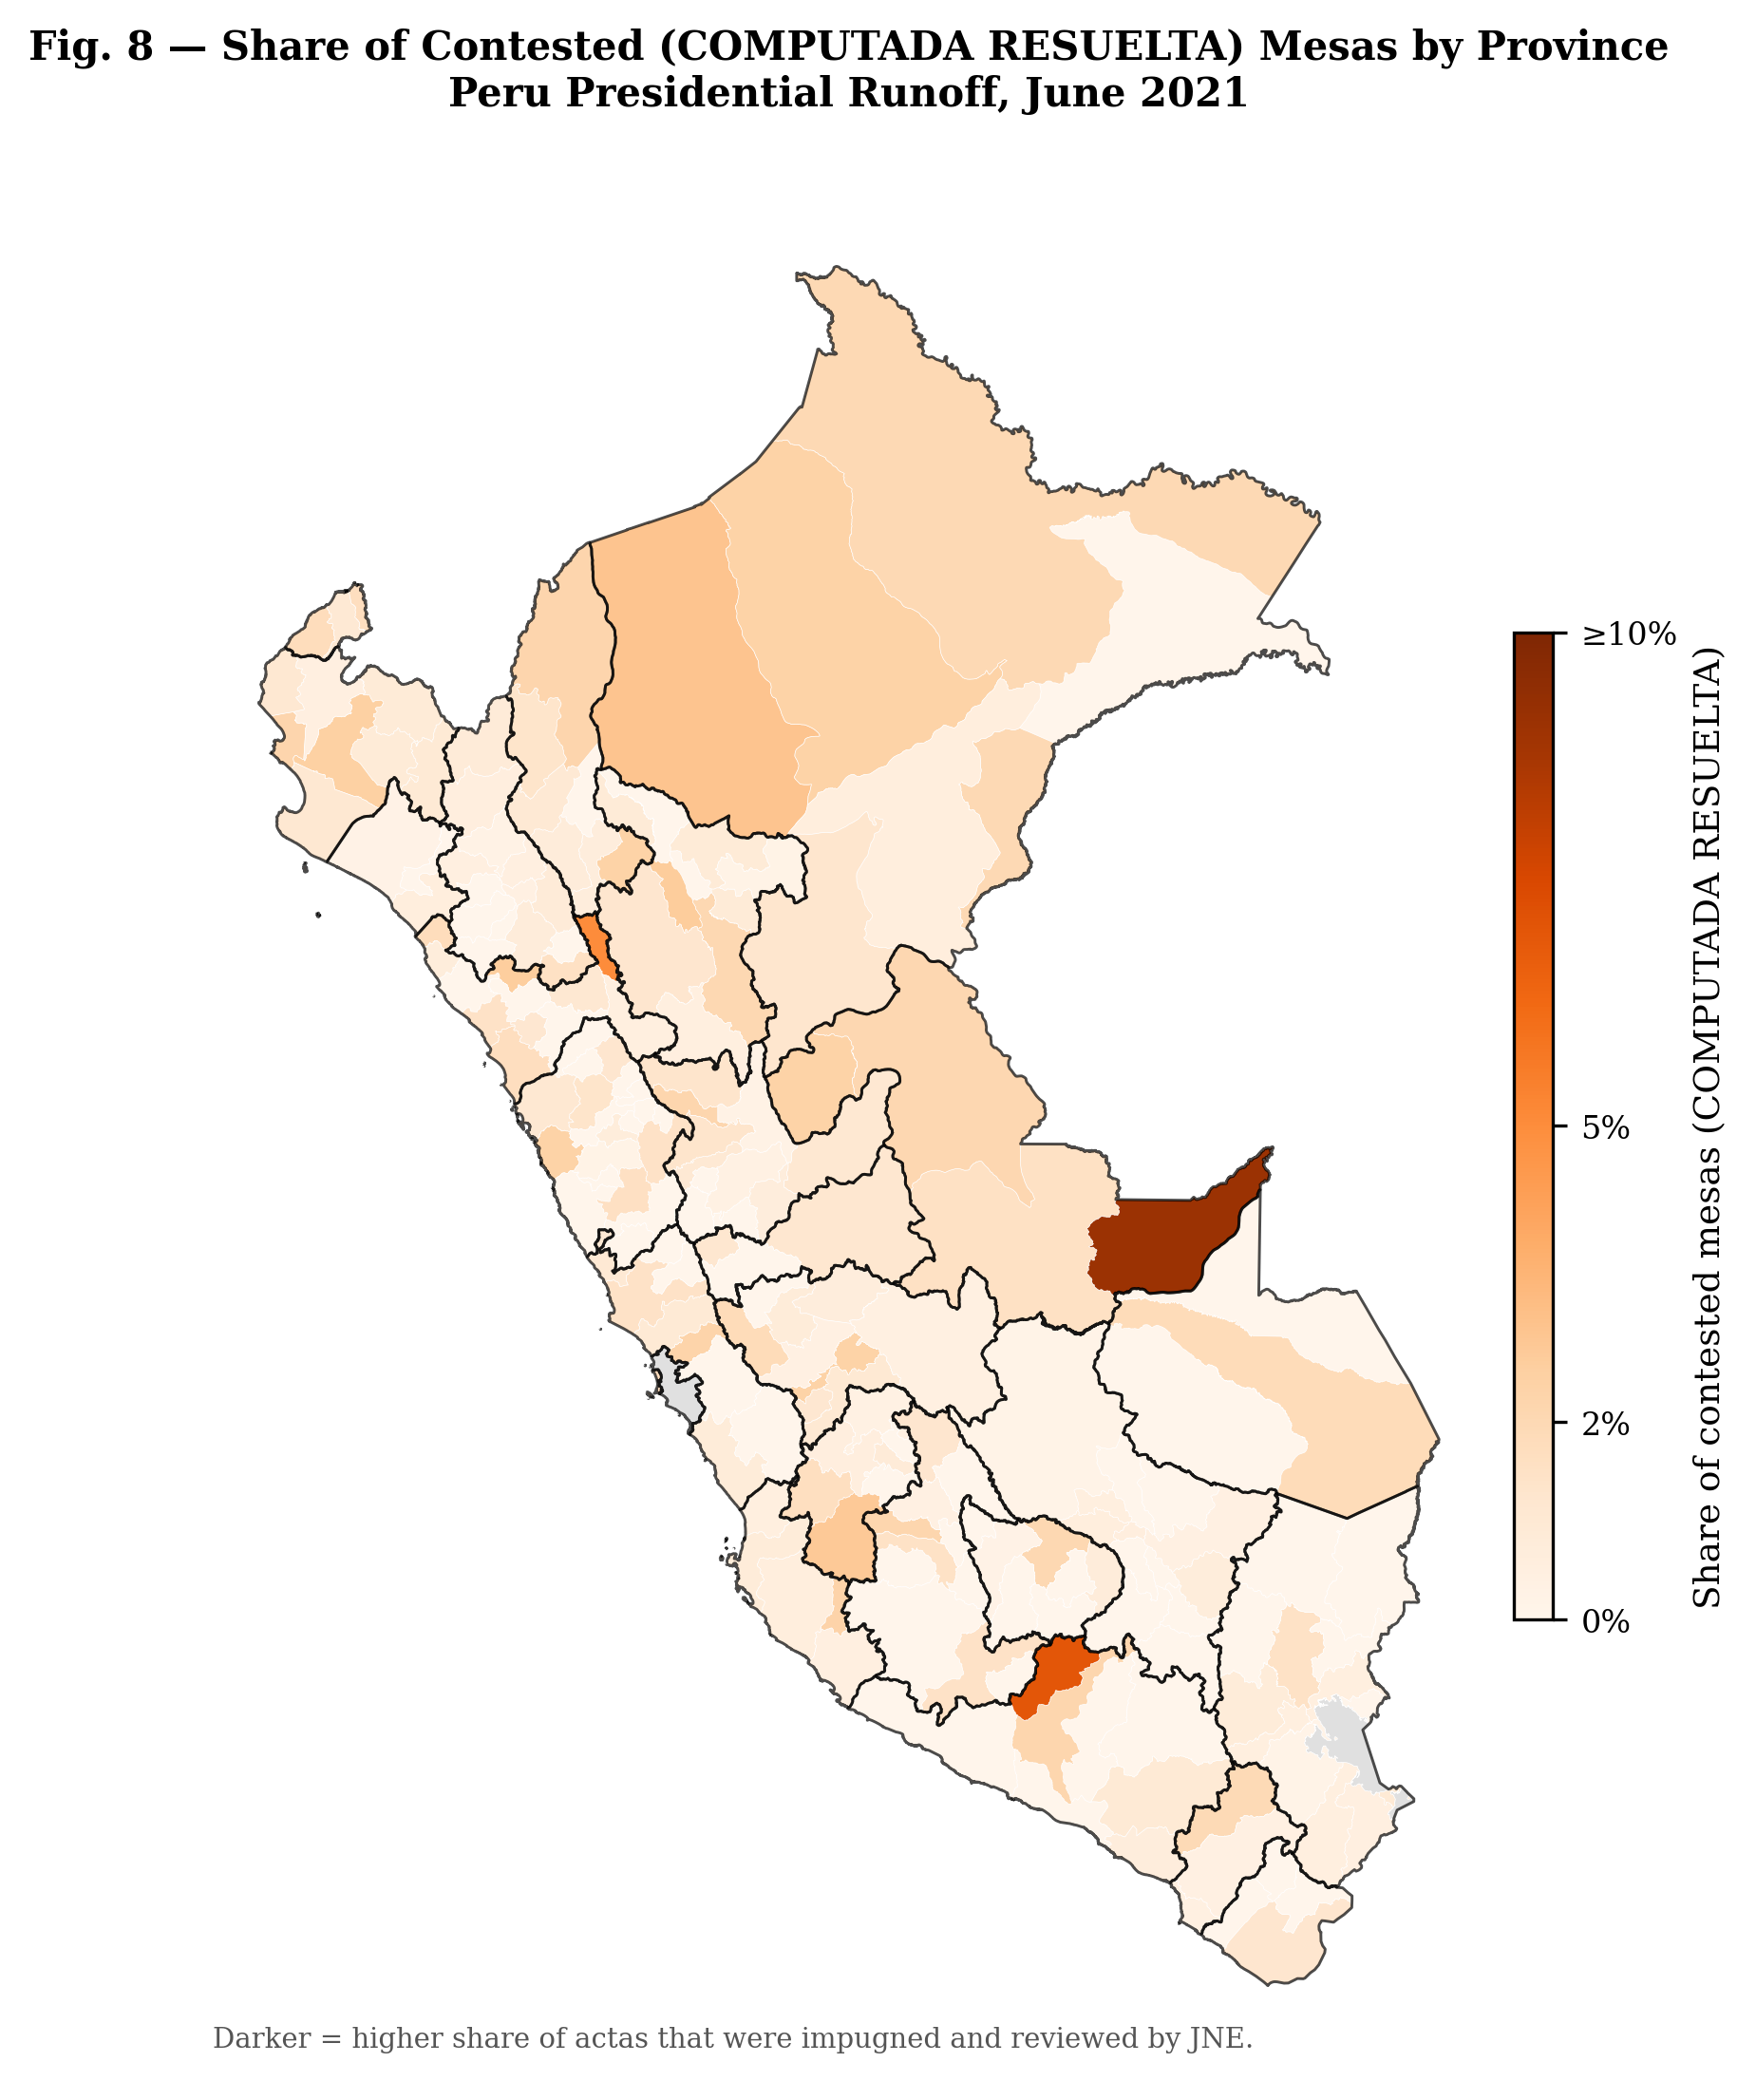
\includegraphics[width=0.88\textwidth]{fig8_map_contested.png}
\caption{Share of contested mesas (COMPUTADA RESUELTA) by province,
         segunda vuelta 2021.
         Darker shading indicates a higher fraction of a province's
         final-status polling stations that were subject to JNE challenge
         and resolution.}
\label{fig:map_contested}
\medskip
\small\textit{Note:} Province-level aggregates from the domestic final-status
sample. Lima province (not Lima region) has the highest contestation share.
\textit{Source:} ONPE \citep{onpe2021}; JNE \citep{jne2021};
GADM 4.1 shapefiles; author's calculations.
\end{figure}

This pattern has a clear institutional explanation. Fujimori's legal team
filed challenges in areas where Fuerza Popular had organizational capacity
to identify procedural violations---primarily the coast and Lima. The JNE
resolved each challenge and incorporated the results, which tilted toward
Fujimori because those polling stations were in Fujimori territory to begin
with. The contested actas reduced Castillo's domestic lead by 39,250 votes.
The claim that they were fraudulently altered \emph{in Castillo's favor} would
require that their true results were even more pro-Fujimori than what the
JNE recorded---and that fraud was concentrated in Fujimori's own strongholds.
No forensic evidence supports this.

\subsection{Distributional fingerprints}

Figure~\ref{fig:klimek} shows the Klimek fingerprint plots for both candidates.
The scatter is organized by macro-region: Sierra mesas cluster in the
upper-right for Castillo (high Castillo share, moderate-to-high turnout) and
in the lower-right for Fujimori; Costa mesas cluster in the lower-right for
Castillo and upper-right for Fujimori; Selva mesas are dispersed between
the two extremes.

\begin{figure}[H]
\centering
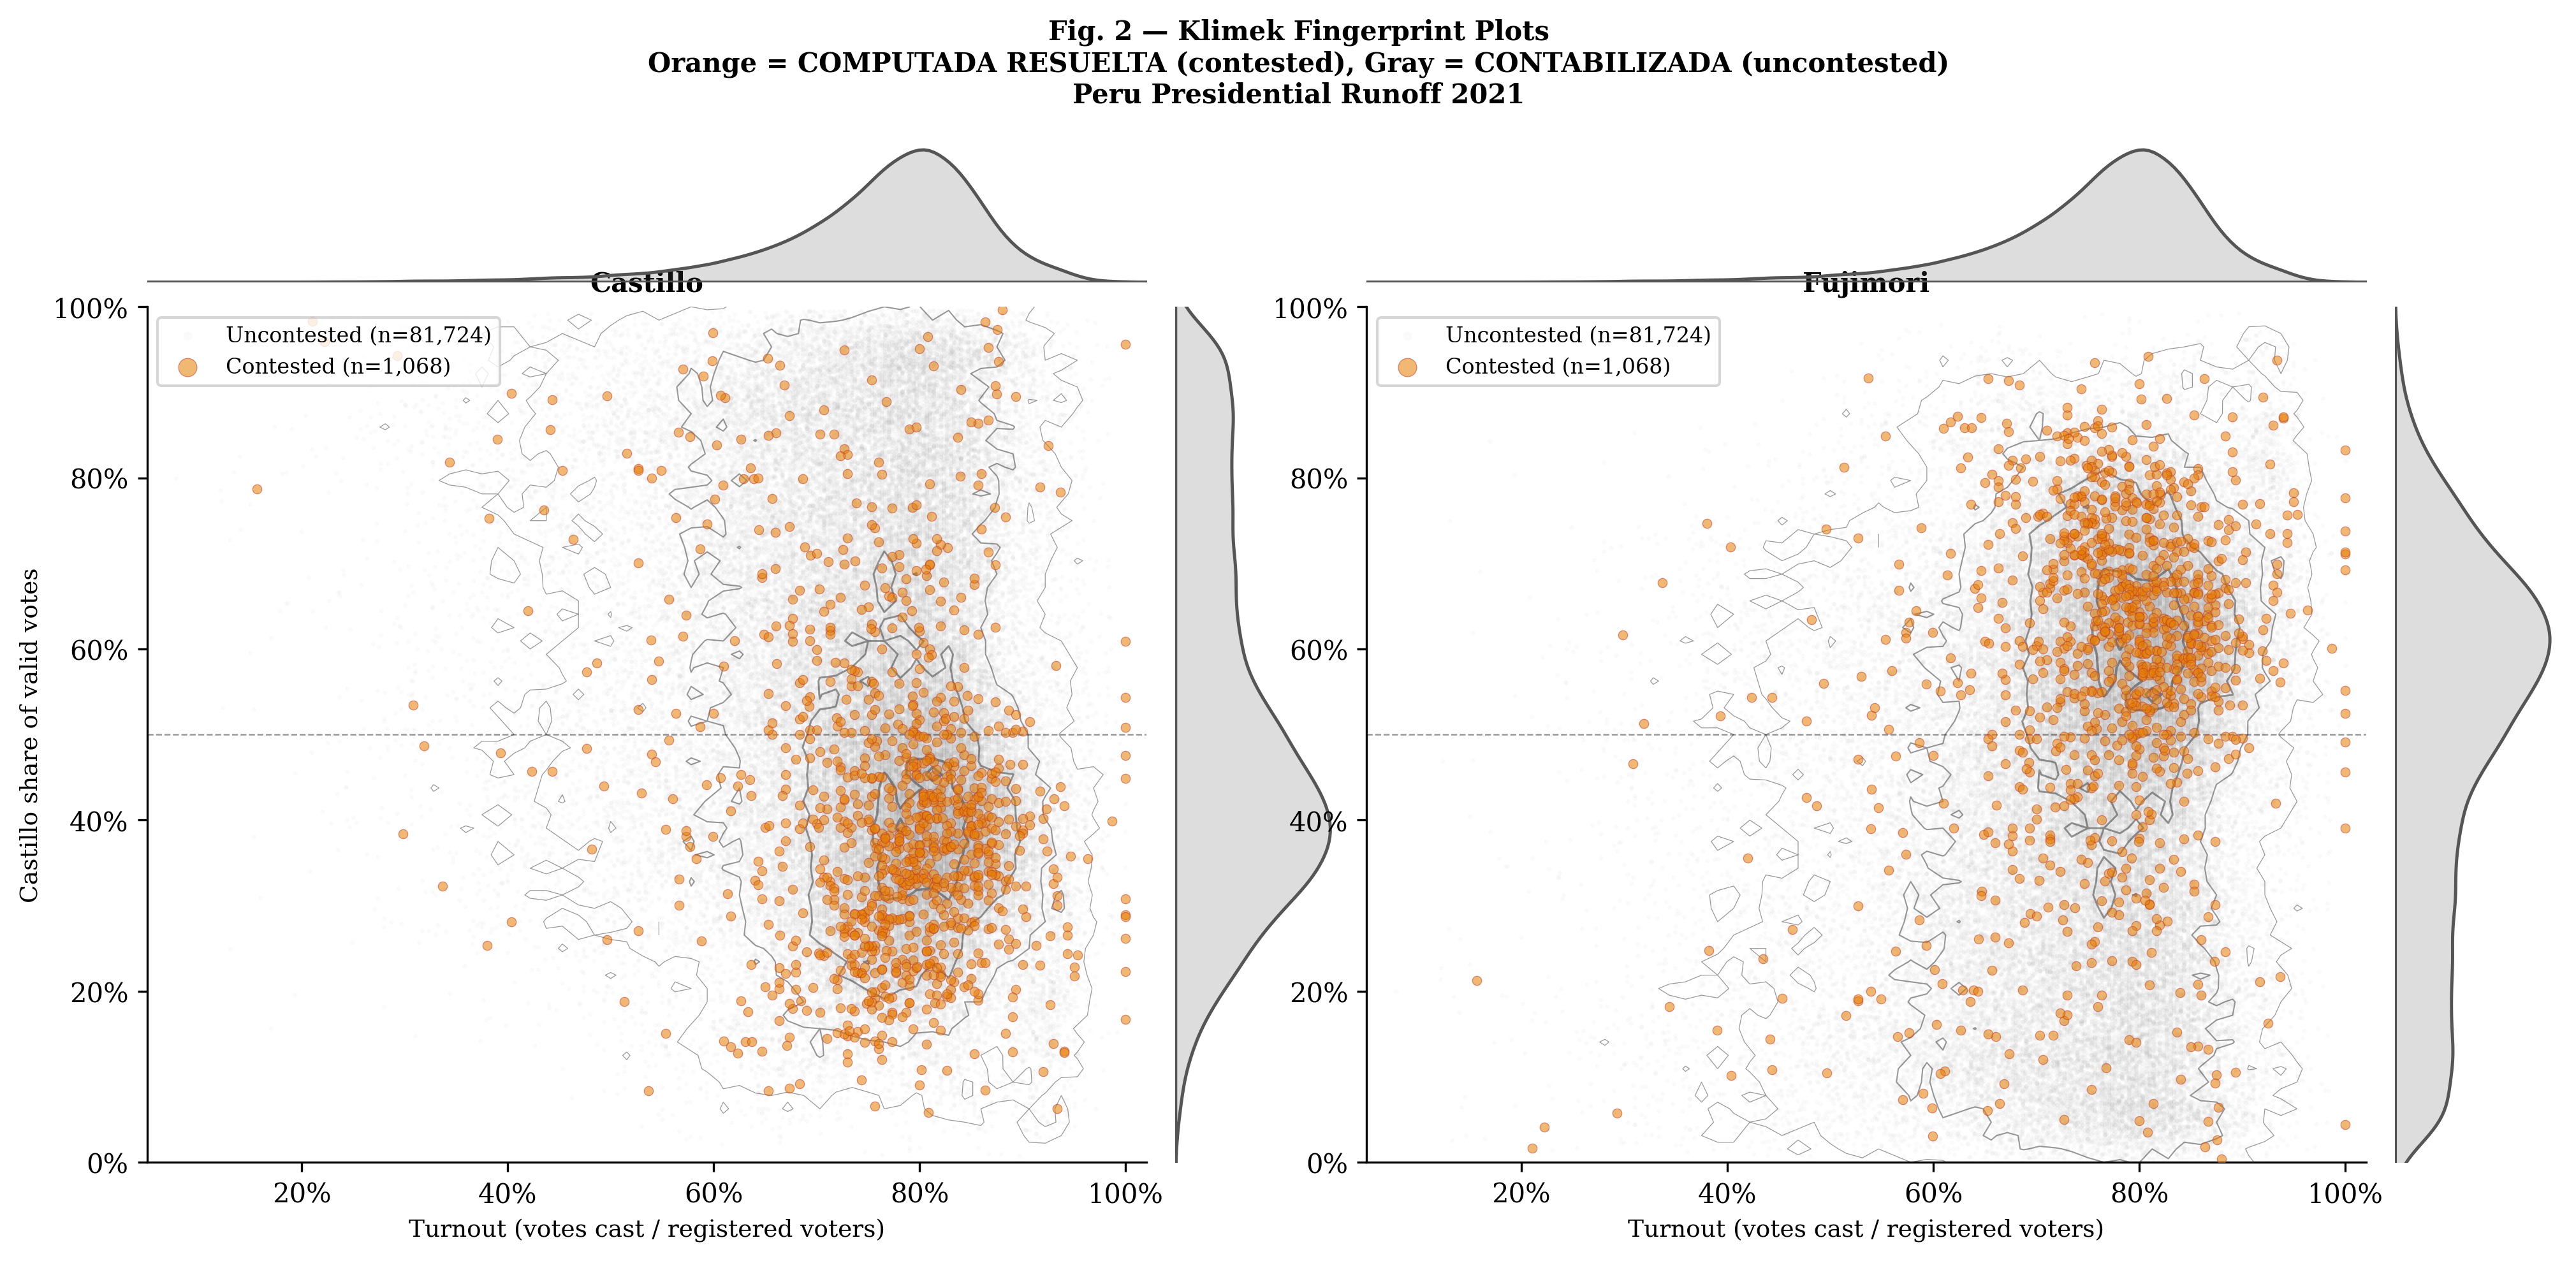
\includegraphics[width=\textwidth]{fig2_klimek.png}
\caption{Distributional fingerprint plots (Klimek et al., 2012).
         Left panel: Castillo vote share on vertical axis.
         Right panel: Fujimori vote share on vertical axis.
         Observations colored by macro-region (Costa = red, Sierra = blue,
         Selva = green). Orange dots are contested mesas (COMPUTADA RESUELTA).
         Density contours overlay the full distribution.}
\label{fig:klimek}
\medskip
\small\textit{Note:} Each dot is one domestic polling station.
The Sierra cluster in the upper-right of the Castillo panel reflects
genuine geographic polarization, not ballot stuffing; it does not extend
as an isolated finger beyond the main distribution.
Orange (contested) dots show no concentration in any corner.
\textit{Source:} ONPE \citep{onpe2021}; author's calculations.
\end{figure}

The key forensic feature is the absence of a ``finger''---a protrusion
extending toward the $(1.0, 1.0)$ corner that \citet{klimek2012} identify as
the ballot-stuffing signature in their Russian benchmarks. The upper-right
region is not empty: there are polling stations with both high turnout
(above 90\,\%) and high Castillo share (above 90\,\%). But these stations
sit \emph{within} the Sierra cluster, which reaches those values throughout.
They are not a separate mode or protrusion; they are the right tail of the
Sierra distribution. The contested mesas (orange dots) are scattered
throughout the cloud with no visible concentration in any corner.

\subsection{Last-digit tests}

Table~\ref{tab:digits} reports the chi-squared tests for all four groups.
All four fail to reject the null hypothesis of uniformity at any conventional
significance level.

\begin{table}[H]
\caption{Last-Digit Uniformity Tests}
\label{tab:digits}
\medskip
\small
\begin{tabular}{lrrrr}
\toprule
Group & $n$ & $\chi^2$ (9 d.f.) & $p$-value & Share digits 0+5 \\
\midrule
Castillo, uncontested & 81,793 & 12.44 & 0.190 & 20.44\,\% \\
Castillo, contested & 1,069 & 4.05 & 0.908 & 18.62\,\% \\
Fujimori, uncontested & 81,724 & 7.84 & 0.551 & 20.11\,\% \\
Fujimori, contested & 1,071 & 4.66 & 0.863 & 20.54\,\% \\
\midrule
Expected under H$_0$ & --- & --- & --- & 20.00\,\% \\
\bottomrule
\end{tabular}
\medskip

\small\textit{Notes:}
The null hypothesis is that last digits are uniformly distributed over $\{0,
1, \ldots, 9\}$. The test excludes observations with zero votes for the
candidate (the last digit is undefined). Zero-exclusions: Castillo uncontested
0, Castillo contested 8, Fujimori uncontested 69, Fujimori contested 6.
None of the four tests rejects uniformity at the 10\,\% level.
The contested subsamples ($n \approx 1{,}070$) have approximately 25\,\% power
to detect heaping at the level observed in documented fraud cases
\citep{beber2012}, so their clean results carry less weight than the
large-sample uncontested results; the uncontested tests have power
exceeding 99\,\% for any practically meaningful departure from uniformity.
\textit{Source:} ONPE \citep{onpe2021}; author's calculations.
\end{table}

For Castillo votes at uncontested mesas ($n = 81{,}793$), the test statistic
is $\chi^2 = 12.44$ ($p = 0.190$). For Fujimori votes at uncontested mesas
($n = 81{,}724$, after dropping 69 mesas with zero Fujimori votes), $\chi^2 =
7.84$ ($p = 0.551$). The contested subsamples are smaller ($n \approx
1{,}070$ each) and therefore have less statistical power, but both also pass
cleanly: $\chi^2 = 4.05$ ($p = 0.908$) for Castillo and $\chi^2 = 4.66$
($p = 0.863$) for Fujimori. The 0+5 digit share---the primary heaping
indicator---ranges from 18.6\,\% to 20.5\,\% across the four groups, all
within half a percentage point of the expected 20\,\%.

\begin{figure}[H]
\centering
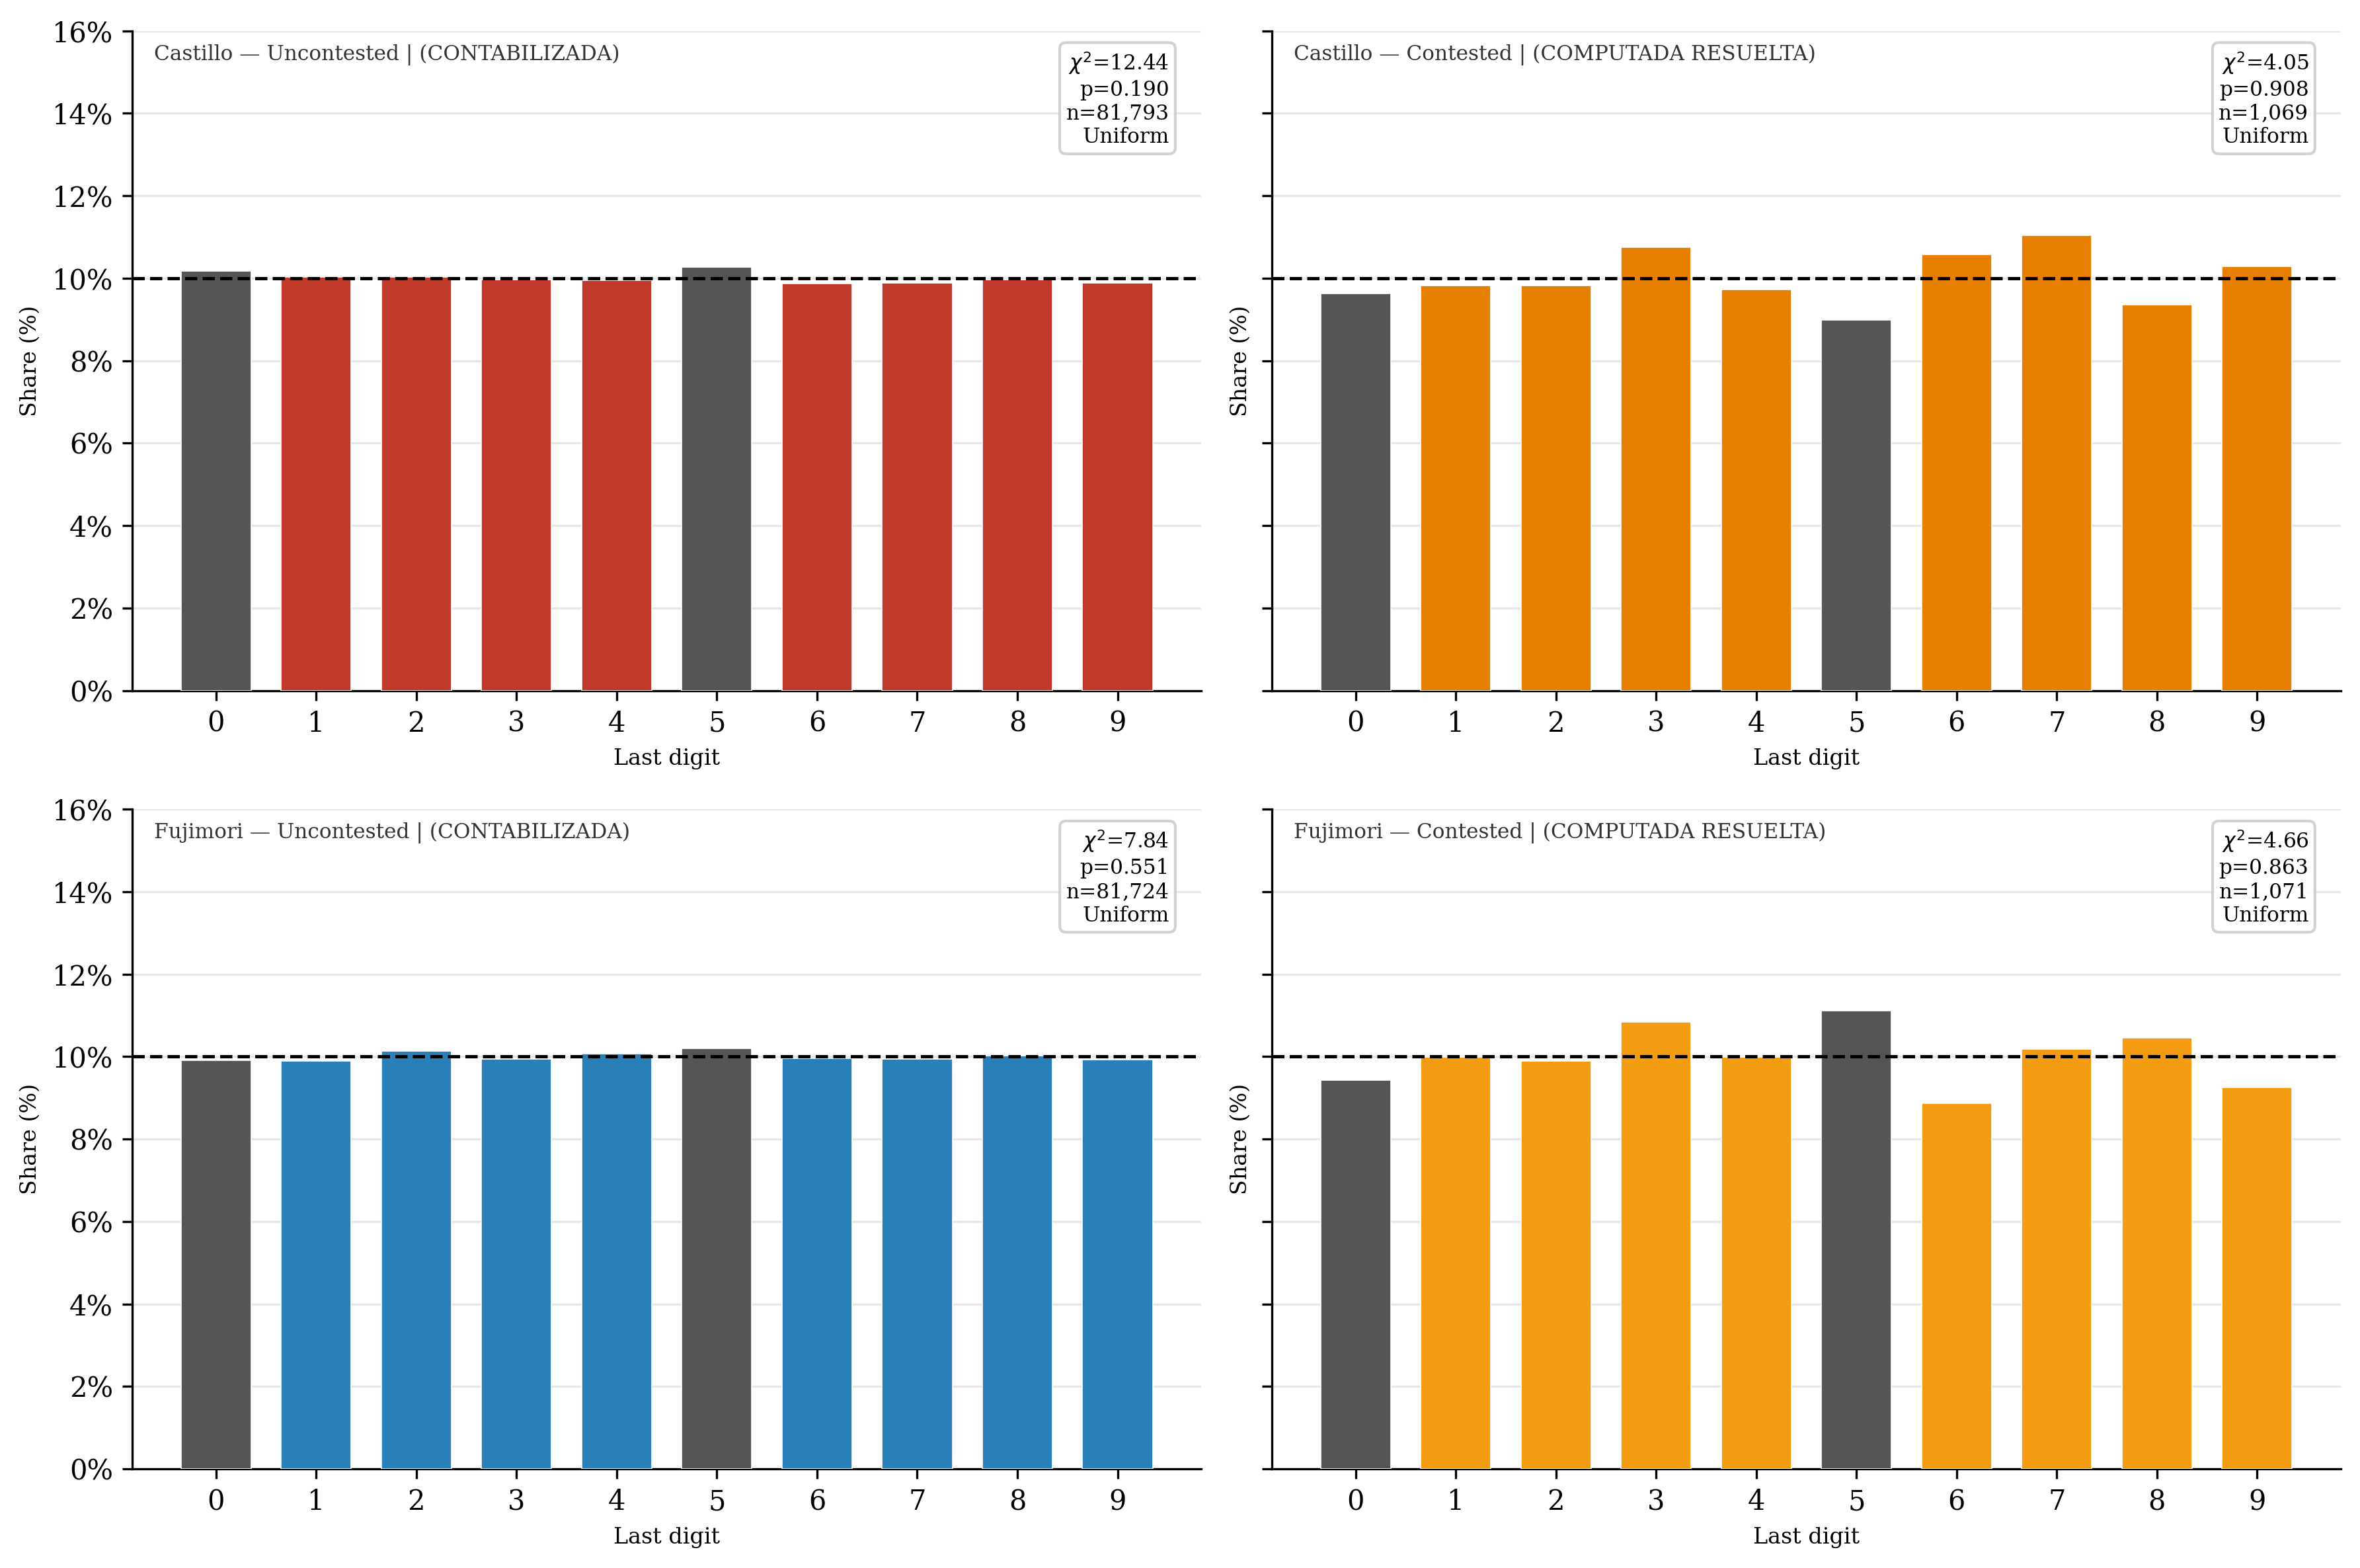
\includegraphics[width=\textwidth]{fig3_lastdigit.png}
\caption{Last-digit distributions for Castillo (left column) and Fujimori
         (right column) votes, separated by polling-station status.
         Top row: uncontested mesas (CONTABILIZADA).
         Bottom row: contested mesas (COMPUTADA RESUELTA).
         Dashed horizontal line at 10\,\% indicates the expected frequency
         under a uniform distribution.}
\label{fig:lastdigit}
\medskip
\small\textit{Note:} Observations with zero votes for the candidate are excluded.
Chi-squared $p$-values: Castillo uncontested 0.190; Castillo contested 0.908;
Fujimori uncontested 0.551; Fujimori contested 0.863.
\textit{Source:} ONPE \citep{onpe2021}; author's calculations.
\end{figure}

Figure~\ref{fig:lastdigit} plots the full digit distributions. Each of the
four panels shows a near-uniform bar chart with no discernible heaping
at 0 or 5. The contested and uncontested distributions are visually
indistinguishable. If vote totals in contested actas had been fabricated
or altered by human actors, last-digit heaping would be the expected
signature. No such pattern appears.

\subsection{Ecological regression}

Table~\ref{tab:regression} reports both specifications.

\begin{table}[H]
\caption{Ecological Regression: First-Round and Second-Round Vote Shares at the District Level}
\label{tab:regression}
\medskip
\small
\begin{tabular}{lcc}
\toprule
 & Specification 1 & Specification 2 \\
 & Eq.~(\ref{eq:spec1}) & Eq.~(\ref{eq:spec2}) \\
\midrule
Constant & 0.392$^{***}$ & 0.393$^{***}$ \\
         & (0.006) & (0.006) \\[4pt]
Primera share (share$_{1v}$) & 0.817$^{***}$ & 0.815$^{***}$ \\
                              & (0.012) & (0.013) \\[4pt]
Share contested (share$_{\text{cont}}$) & & $-$0.113 \\
                                         & & (0.253) \\[4pt]
Primera $\times$ contested & & 0.231 \\
                            & & (0.614) \\[4pt]
\midrule
$N$ & 1,873 & 1,873 \\
$R^2$ & 0.708 & 0.708 \\
\bottomrule
\end{tabular}
\medskip

\small\textit{Notes:}
Dependent variable: Castillo valid-vote share in the segunda vuelta,
aggregated to the district level. Primera share is Peru Libre's valid-vote
share in the primera vuelta (candidate 16, VOTOS\_P16).
Share contested is the fraction of a district's final-status segunda vuelta
mesas that are \emph{computada resuelta}. HC0-robust standard errors
in parentheses. $^{***}$ $p < 0.001$.
Sample restricted to districts with at least 10 valid votes in the segunda
vuelta and positive Peru Libre votes in the primera vuelta. Districts with
at least one contested mesa: 314 (16.8\,\% of sample).
\textit{Source:} ONPE \citep{onpe2021, onpe2021a}; author's calculations.
\end{table}

Specification~1 regresses Castillo's second-round district share on Peru
Libre's first-round district share across $N = 1{,}873$ districts with
matched data. The estimated relationship is:
\[
  \widehat{\text{share}}_{2v} = 0.392 + 0.817 \times \text{share}_{1v},
  \quad R^2 = 0.708.
\]
The slope of 0.817 is less than 1: in districts where Peru Libre was
strong in the first round, Castillo gained proportionally but not one-for-one,
reflecting the fact that many additional votes came from former supporters
of other first-round candidates rather than simple mobilization of the
existing Peru Libre base. The intercept of 0.39 confirms that Castillo
drew substantial anti-Fujimori votes even in districts where Peru Libre had
minimal first-round presence. The $R^2$ of 0.71 indicates that
first-round geography explains most of the variation in second-round outcomes.

\begin{figure}[H]
\centering
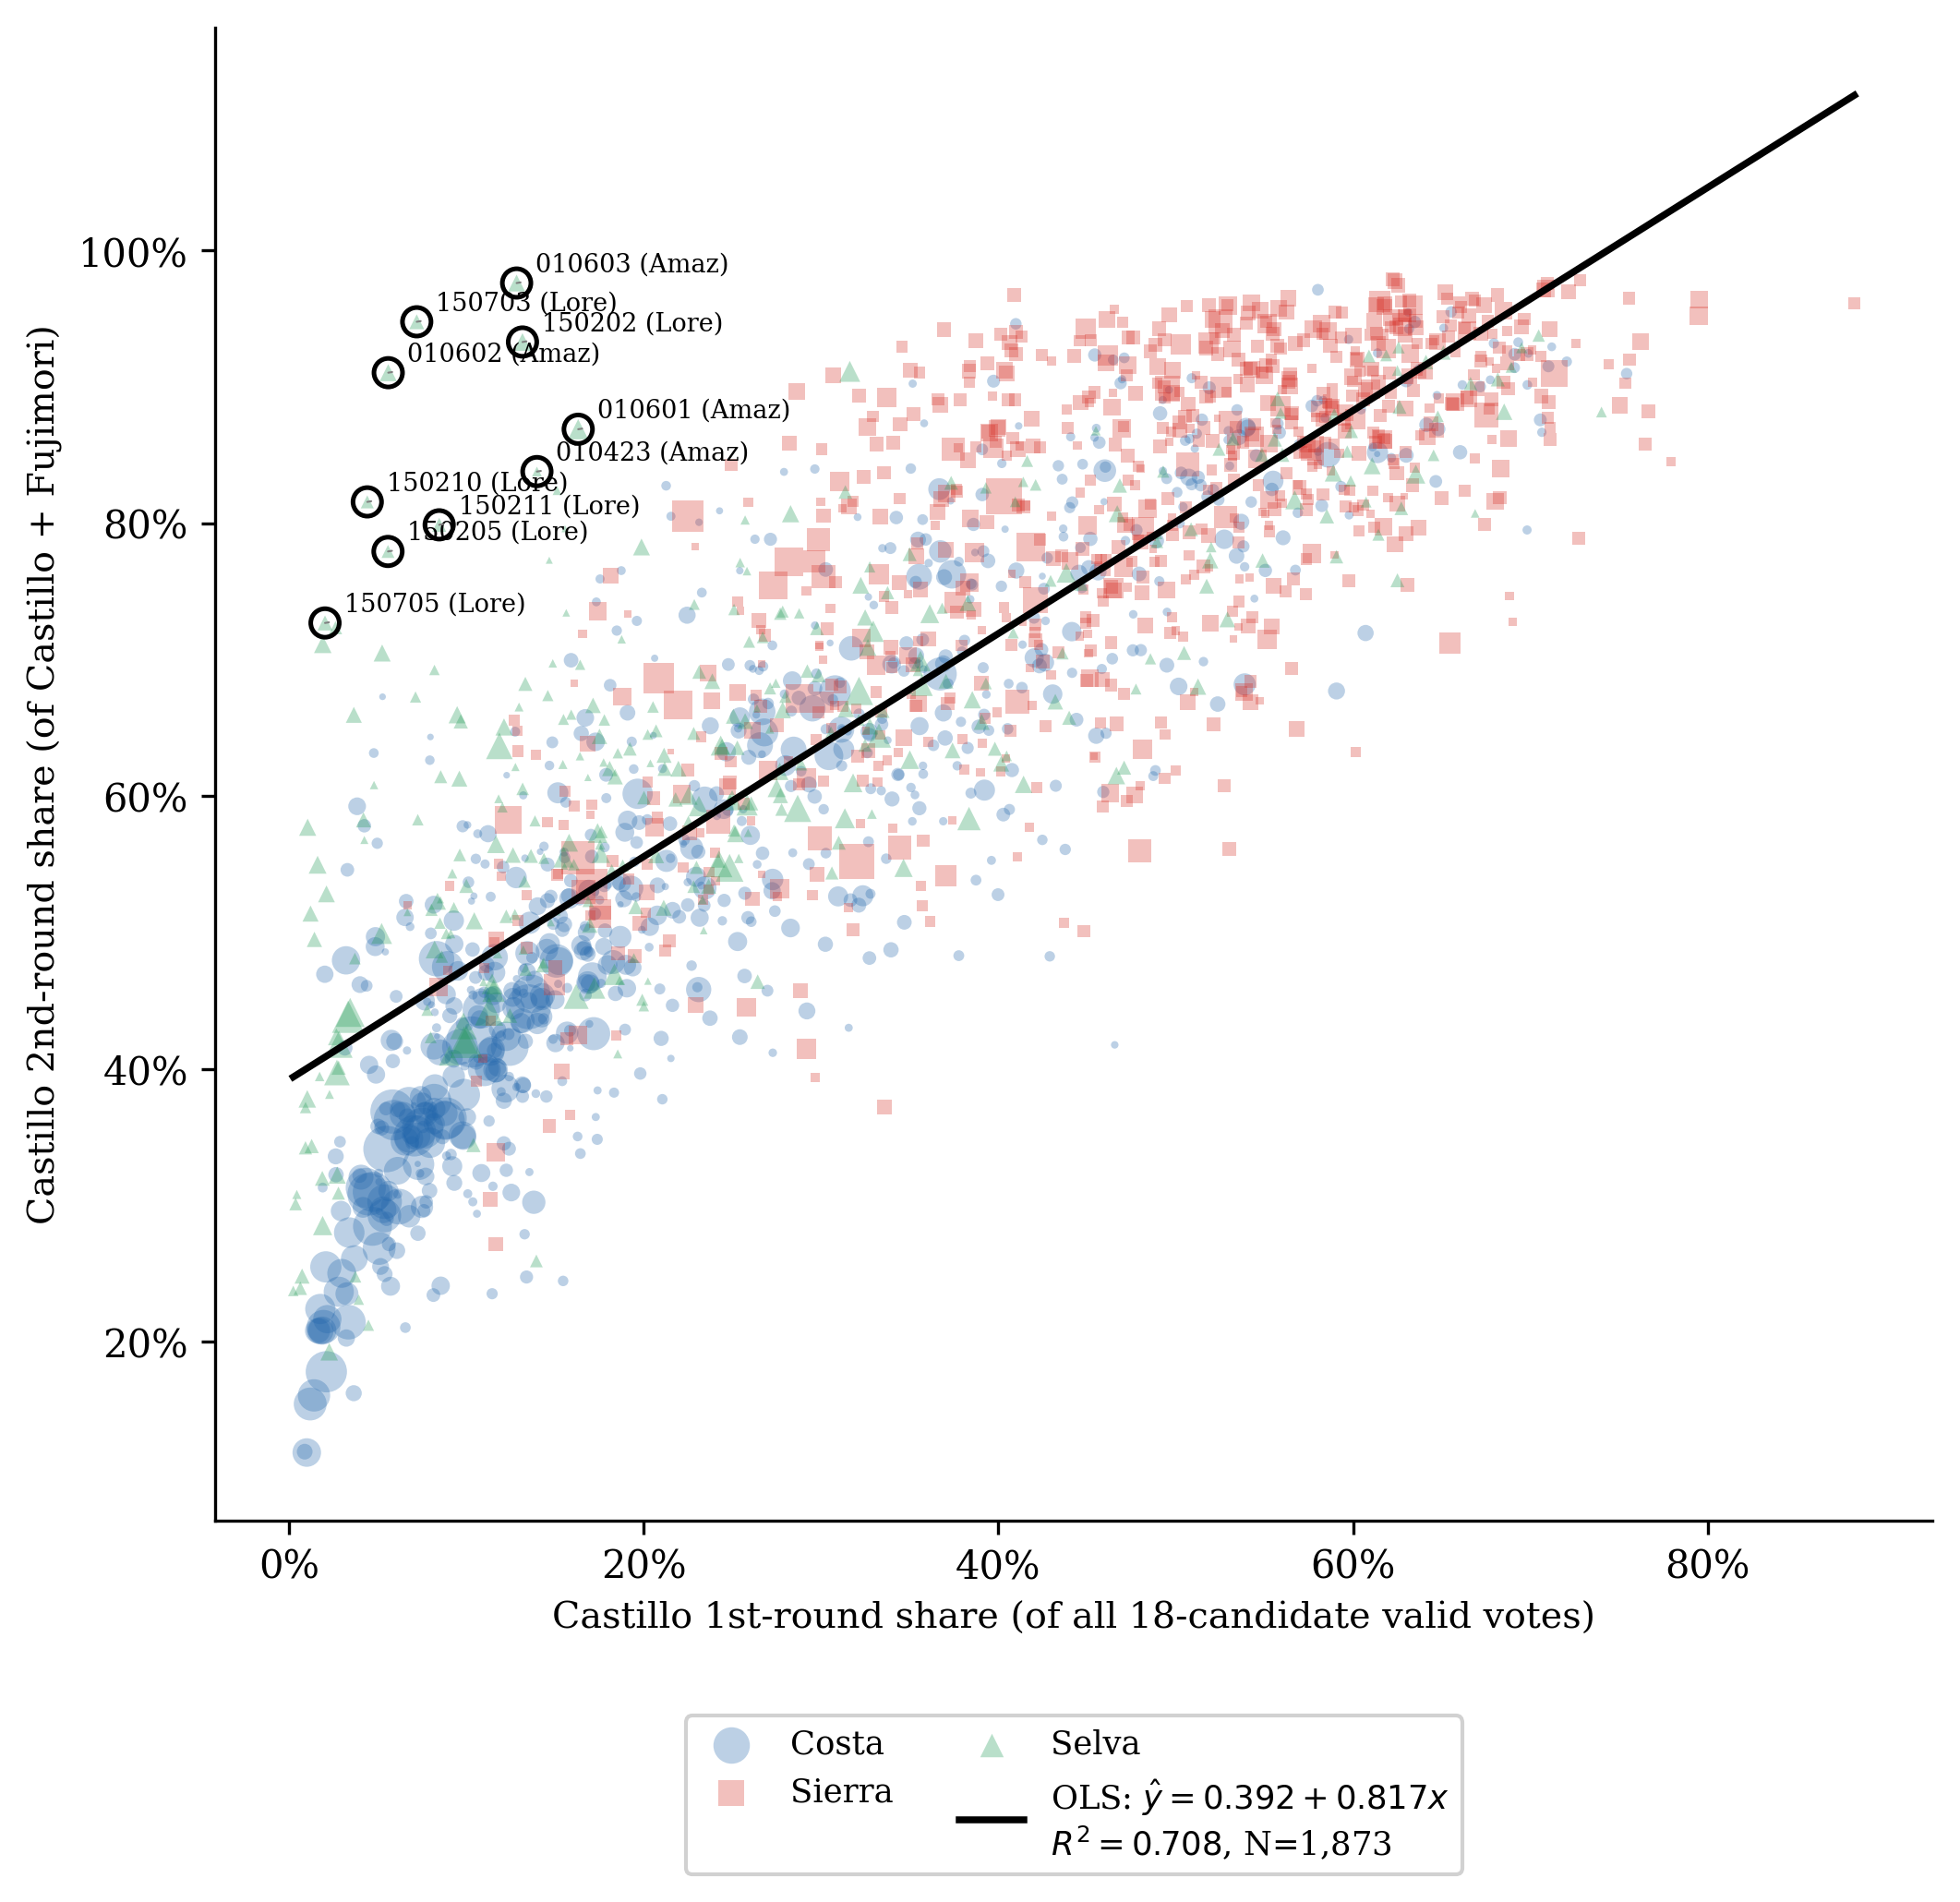
\includegraphics[width=0.80\textwidth]{fig4_primera_vs_segunda.png}
\caption{First-round (primera vuelta) vs.\ second-round (segunda vuelta)
         Castillo/Peru Libre vote share at the district level.
         Each point is one of 1,873 districts. The fitted line is from
         Specification~1 of Table~\ref{tab:regression}. Orange points
         are districts with any contested (COMPUTADA RESUELTA) mesas.}
\label{fig:primera_segunda}
\medskip
\small\textit{Note:} Districts with fewer than 10 valid segunda vuelta votes
or zero primera vuelta Peru Libre votes are excluded.
The top-10 positive-residual districts are in Loreto and Amazonas,
which have high geographic isolation; none are in the departments
identified in Fujimori's fraud allegations.
\textit{Source:} ONPE \citep{onpe2021, onpe2021a}; author's calculations.
\end{figure}

Figure~\ref{fig:primera_segunda} displays the district-level scatter with the
fitted regression line. The relationship is tight and linear, with no obvious
outliers or breaks. The districts with the largest positive residuals
(where Castillo most over-performed relative to first-round prediction)
are concentrated in Loreto and Amazonas departments---remote Amazonian
areas with historically variable turnout and high geographic isolation,
not departments identified in the fraud allegations.

Specification~2 adds the district share of contested mesas
($\text{share\_cont}_d$) and its interaction with first-round share. Neither
coefficient is statistically significant: $\hat{\gamma} = -0.113$
($\text{SE} = 0.253$, $p = 0.656$) and $\hat{\delta} = 0.231$
($\text{SE} = 0.614$, $p = 0.707$). The $R^2$ is unchanged at 0.708.
Districts with a higher concentration of contested mesas do not
over-perform for Castillo after conditioning on first-round baseline.

\subsection{Turnout patterns}

Figure~\ref{fig:turnout} shows the turnout distributions for both rounds.
Average domestic turnout in the segunda vuelta was 76.1\,\%, down from the
primera vuelta. This directional finding runs against what ballot stuffing
would produce: adding fabricated votes to tallies would inflate recorded
turnout, generating a distribution shifted toward the high end. The segunda
vuelta distribution is unimodal and roughly symmetric, with no secondary peak
near 100\,\% that would suggest mass turnout manipulation.

\begin{figure}[H]
\centering
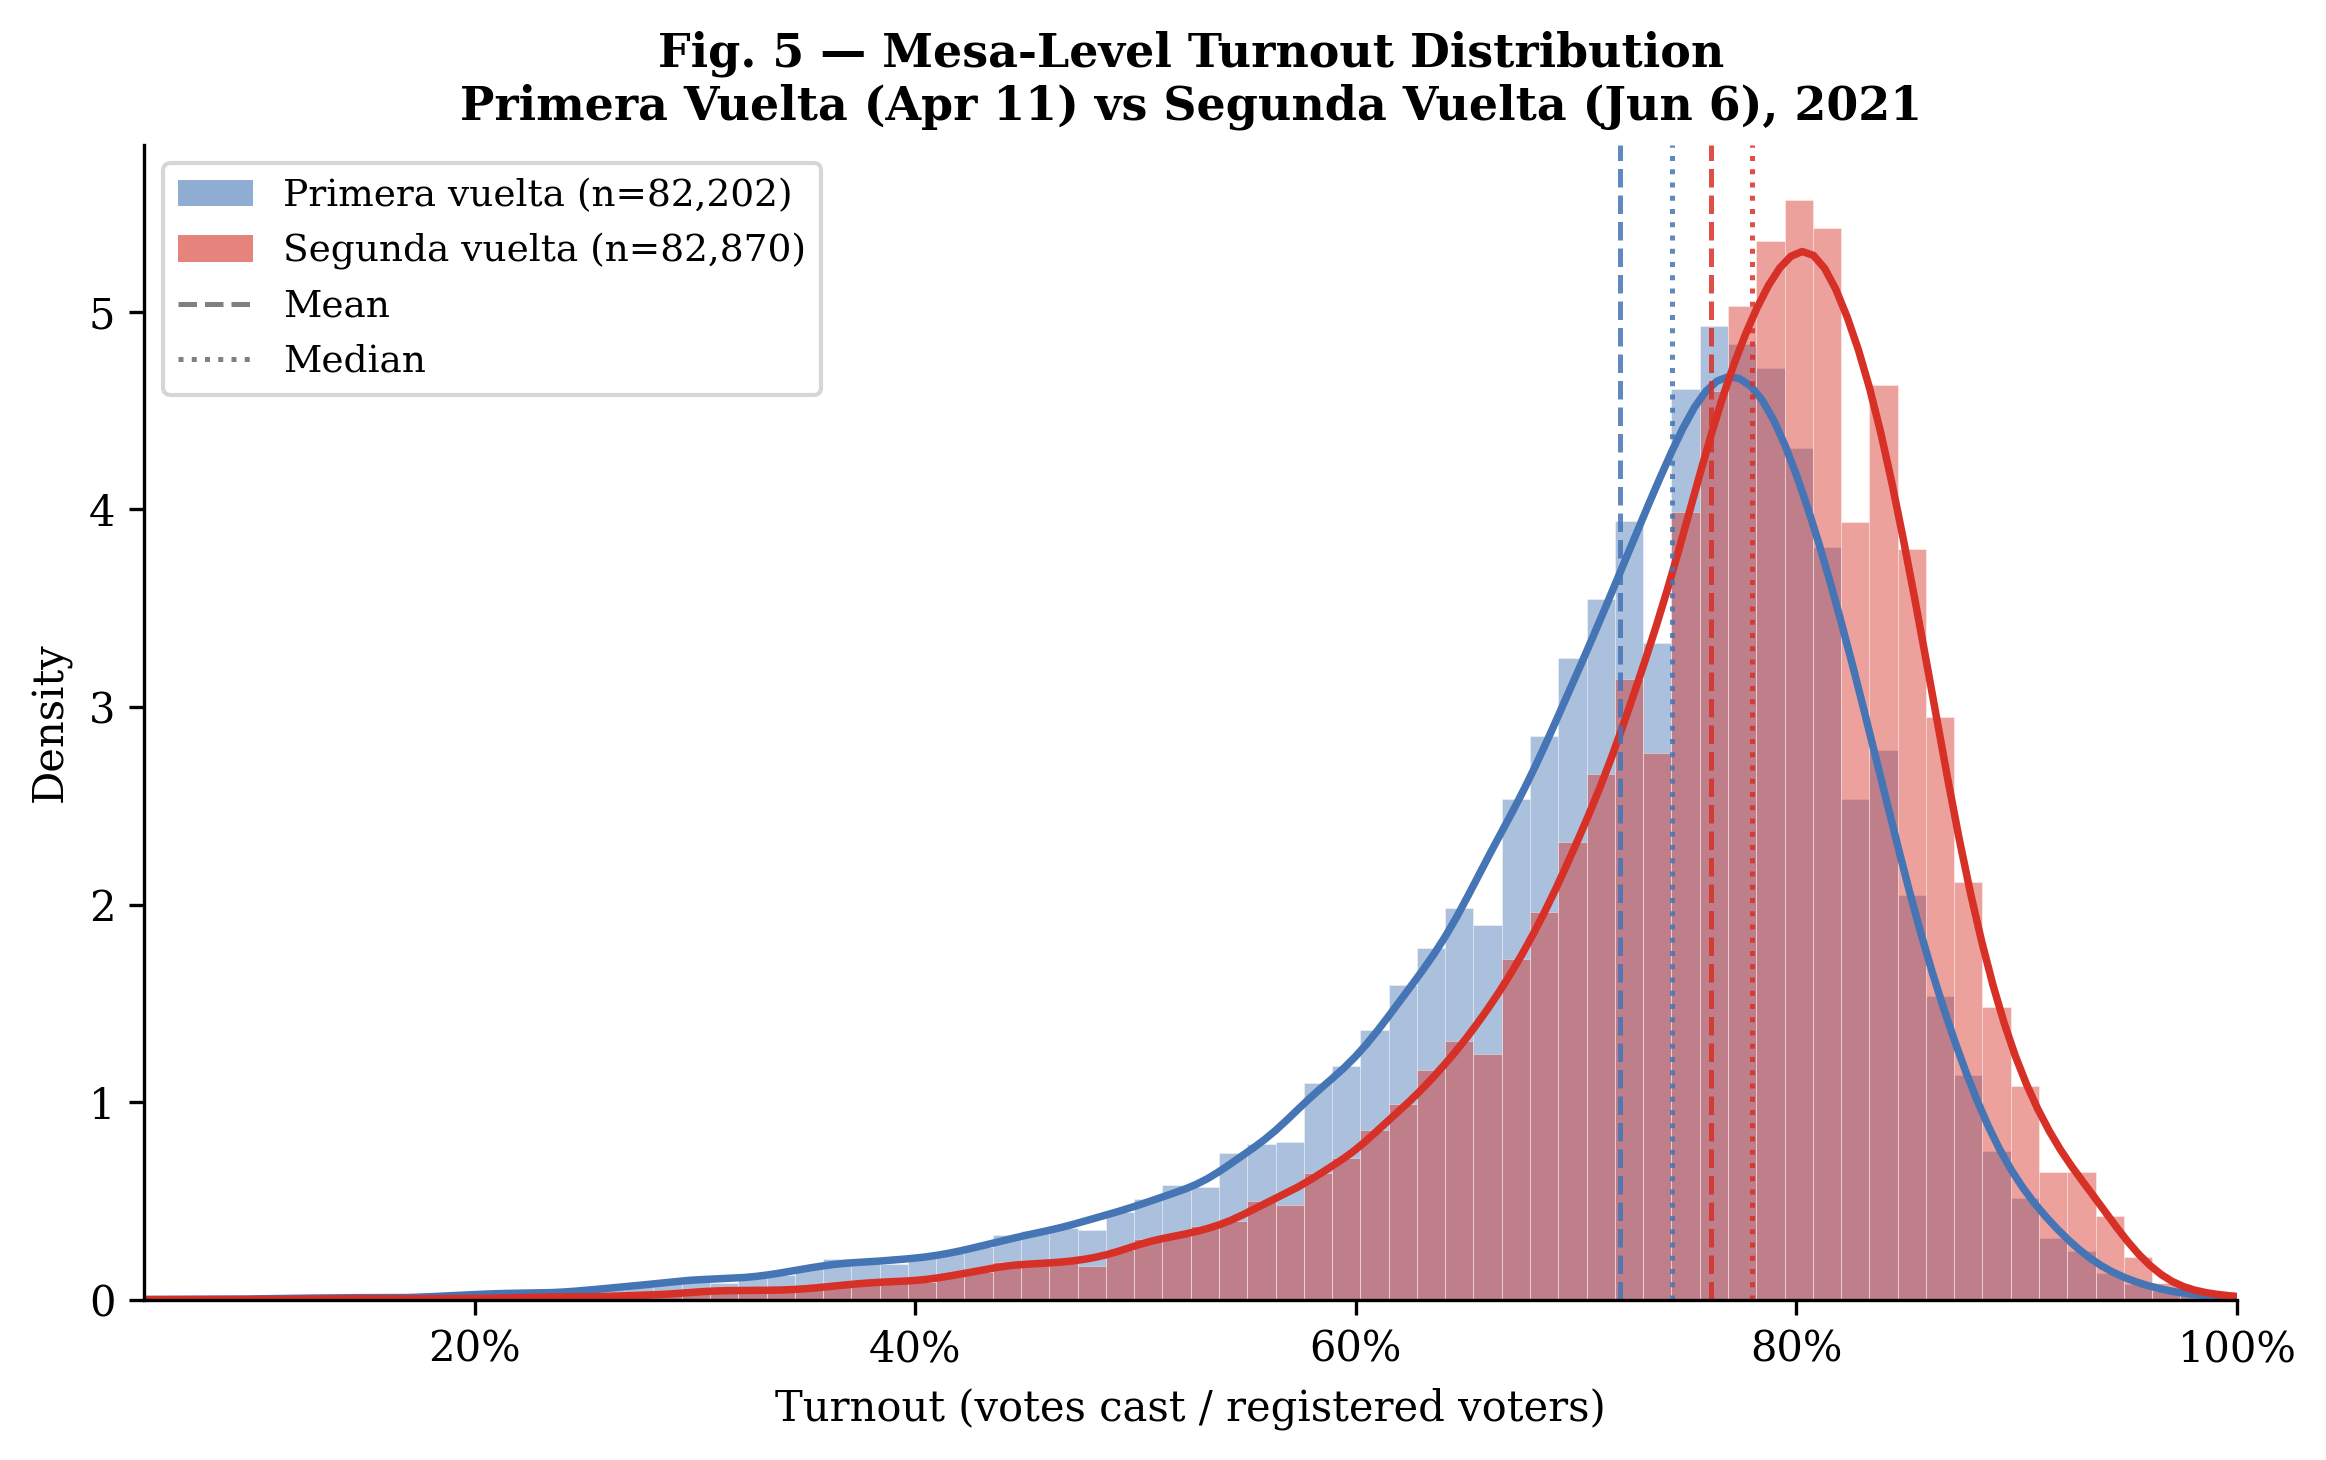
\includegraphics[width=0.85\textwidth]{fig5_turnout_dist.png}
\caption{Turnout distribution by polling station, primera vuelta (April 2021)
         and segunda vuelta (June 2021).
         Vertical lines mark the respective medians.}
\label{fig:turnout}
\medskip
\small\textit{Note:} Domestic final-status samples for each round,
with turnout clipped at 1.05 for display purposes.
\textit{Source:} ONPE \citep{onpe2021, onpe2021a}; author's calculations.
\end{figure}

The anomaly flag counts in Table~\ref{tab:flags} are consistent with this
picture. Zero mesas exceed 100\,\% turnout. Only 2 mesas fall below 10\,\%
turnout (both are small rural mesas with a single registered-voter
discrepancy). There are 57 mesas with turnout above 98\,\%---none show
the accompanying perfect or near-perfect vote shares that would mark
ballot stuffing.

\subsection{Null vote geography}

Figure~\ref{fig:map_nullvotes} maps the provincial null-vote rate.

\begin{figure}[H]
\centering
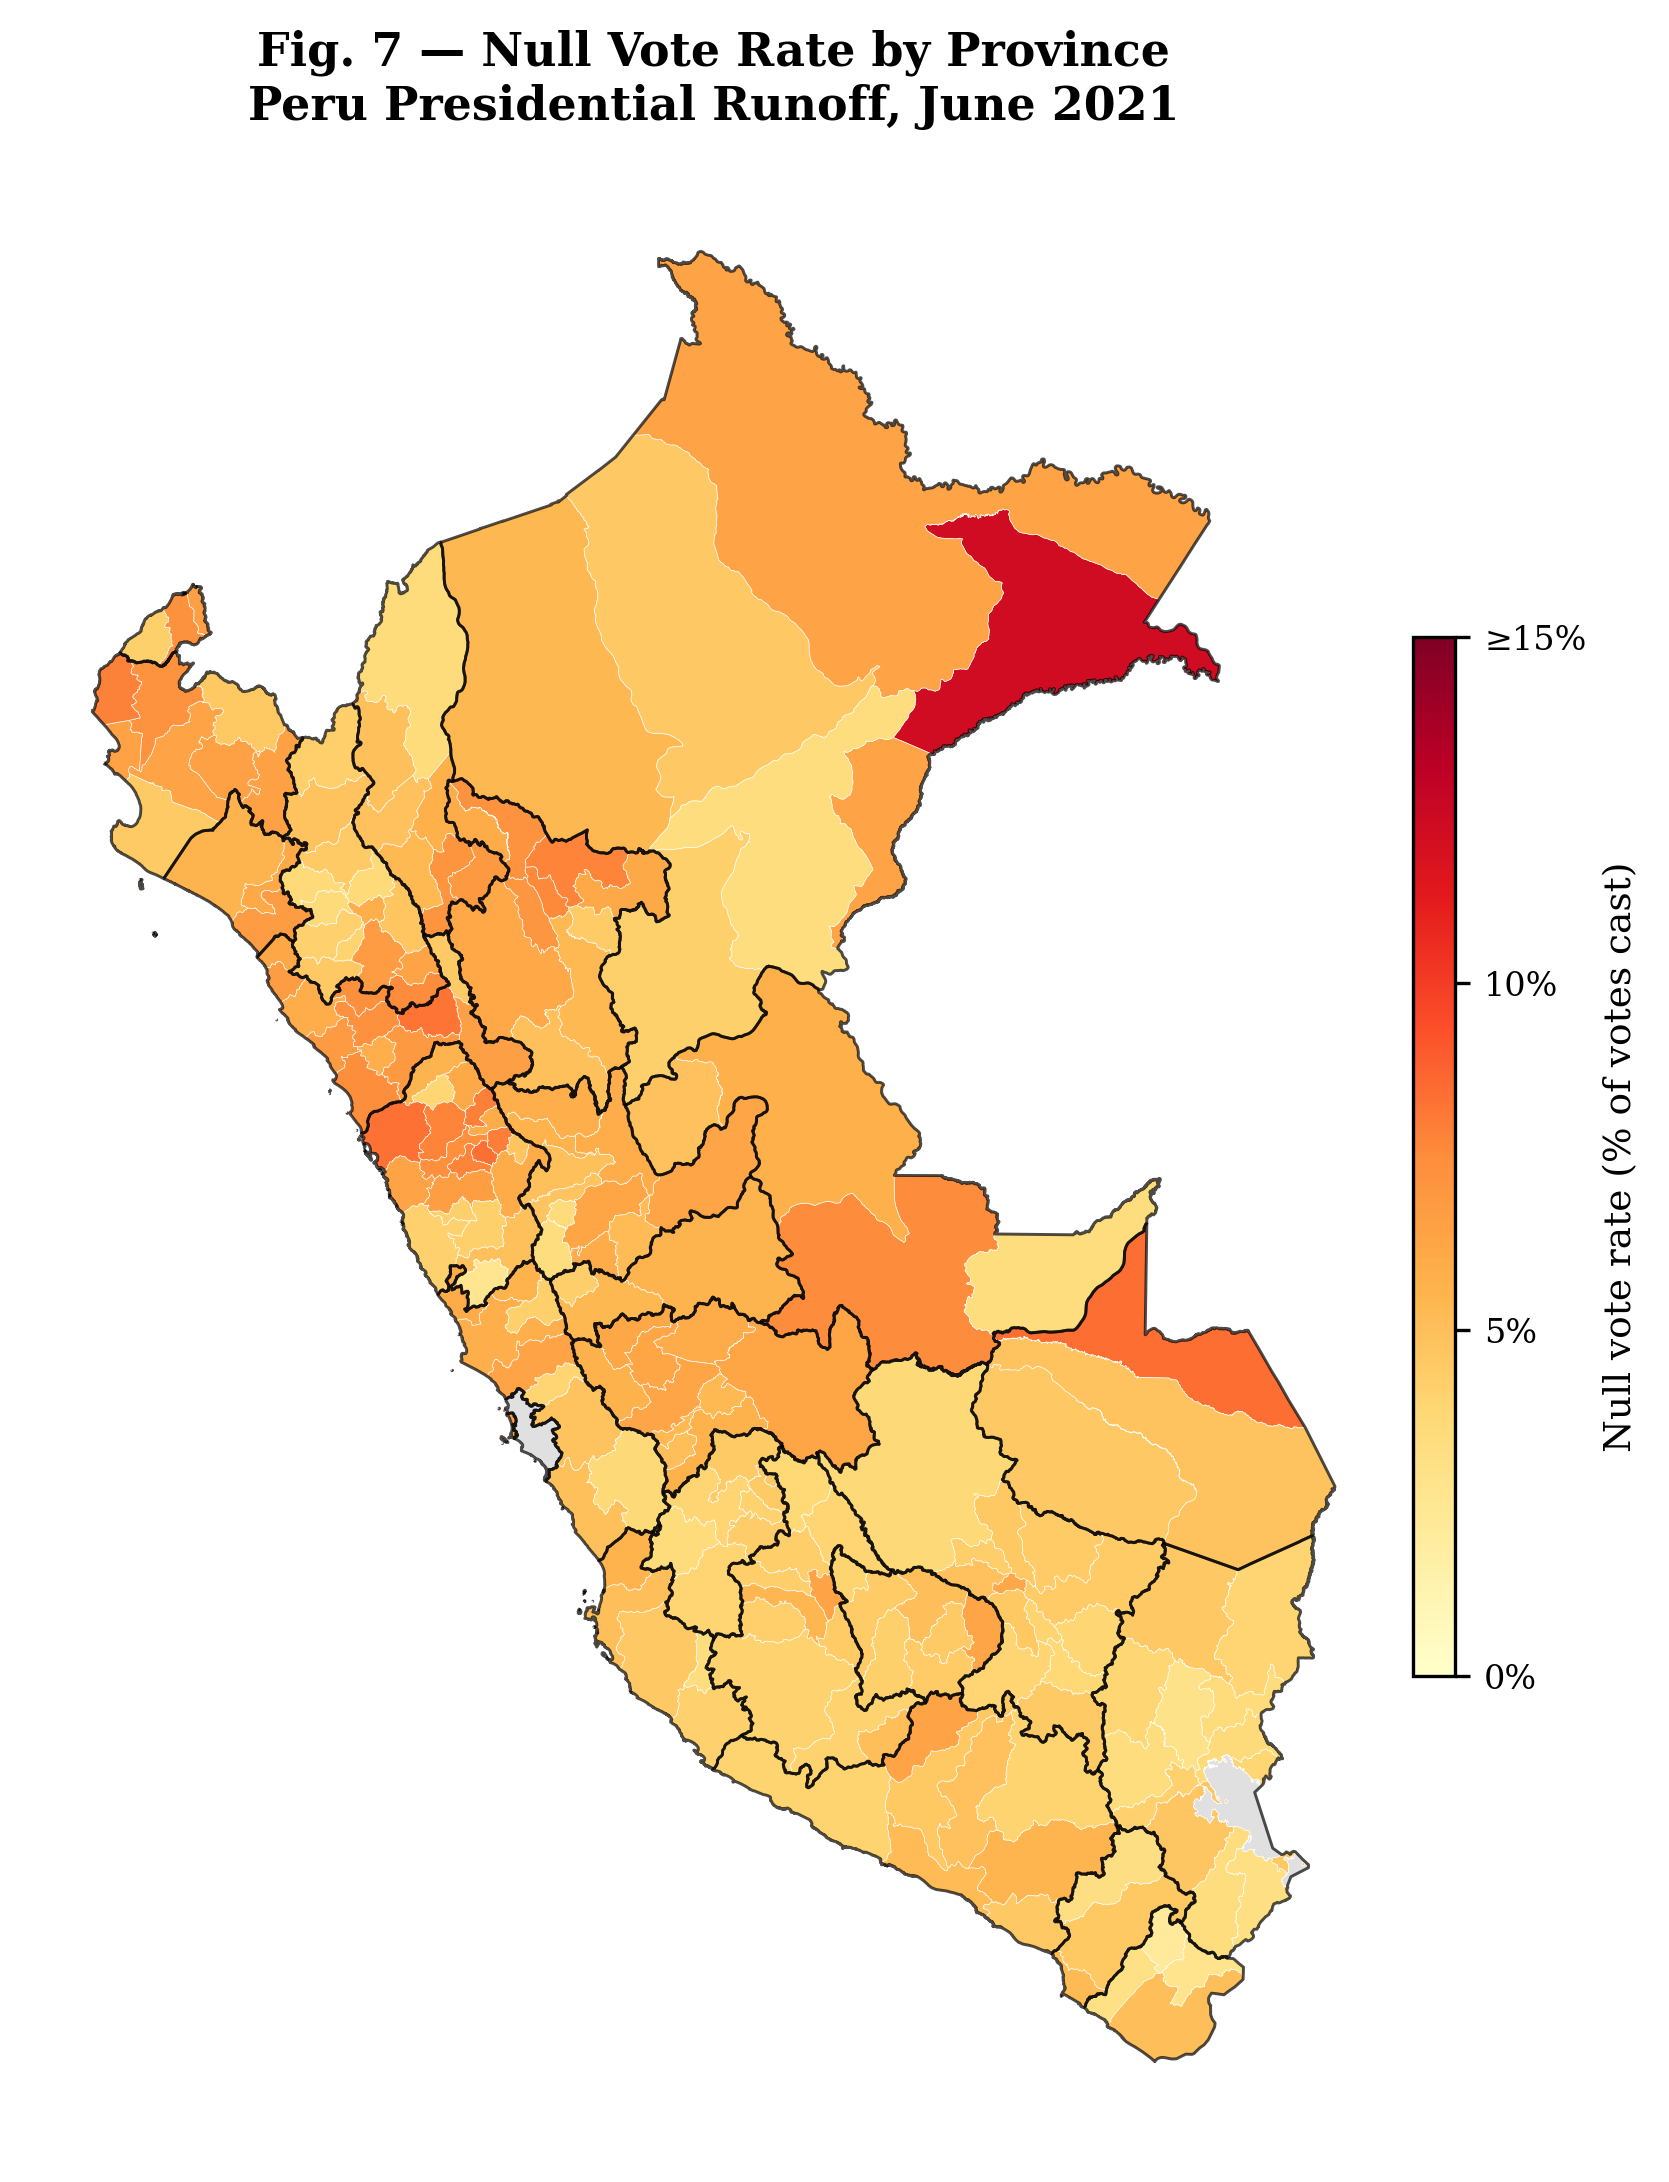
\includegraphics[width=0.88\textwidth]{fig7_map_nullvotes.png}
\caption{Null vote rate by province (null votes as a share of total votes cast),
         segunda vuelta 2021.
         Darker shading indicates higher null rates.}
\label{fig:map_nullvotes}
\medskip
\small\textit{Note:} Province-level aggregates from the domestic final-status
sample. Null votes (VOTOS\_VN) include all ballots invalidated at the
polling station during counting.
\textit{Source:} ONPE \citep{onpe2021}; GADM 4.1 shapefiles; author's calculations.
\end{figure}

High null rates concentrate in coastal and metropolitan areas: Lima
(the capital), Piura, La Libertad, and Lambayeque all show elevated
null vote rates. These are Fujimori's strongest departments. If fraud
had taken the form of systematic invalidation of pro-Castillo votes,
null rates would be elevated in Castillo's highland strongholds. The
observed pattern points instead to protest voting by urban Lime\~nos
who disliked both candidates---a plausible behavioral response given
the polarizing choice on offer.

% =============================================================================
\section{Discussion}
\label{sec:discussion}
% =============================================================================

\subsection{Why fraud allegations gained traction}

Three factors explain why Fujimori's fraud narrative resonated despite the
absence of supporting evidence. First, the margin was historically narrow.
At 44,263 votes out of 17 million cast, any irregularity in a few hundred
polling stations could, in principle, have been decisive. Close elections
generate fraud allegations in many countries \citep{lehoucq2003}, and Peru
was no exception.

Second, the geographic pattern of results appeared anomalous to urban
observers unfamiliar with the political geography of the Peruvian sierra.
Vote shares of 80--90\,\% for a single candidate in polling stations with
near-universal turnout look like fraud to someone who has never visited
these regions and does not know their voting history. In Andean communities
with strong collective identities and long histories of political mobilization,
near-unanimous results are not unusual and do not require manipulation.

Third, and most consequential for the fraud narrative, the running count
shifted toward Castillo over several days as highland actas arrived later
than urban ones. This is the ``early-count mirage'' documented by
\citet{idrobo2022} for Bolivia 2019: urban precincts count faster, early
returns favor the urban candidate (Fujimori), and as rural results arrive
the lead shifts. The shift is a mechanical consequence of differential
reporting speeds in a geographically polarized electorate. It is not
suspicious, but it is visible, and it was interpreted by Fujimori's supporters
as evidence that votes were being added to Castillo's total after the
initial count.

A fourth factor was Fujimori's personal legal exposure. She faced ongoing
criminal prosecution for corruption and illegal campaign financing at the
time of the election. A Castillo presidency increased the probability that
she would be convicted and imprisoned.
This gave her a rational personal incentive to contest the result beyond
what the evidence warranted, independent of any genuine belief that fraud
had occurred.

\subsection{Comparison with Bolivia 2019}

The Bolivia 2019 election offers the closest methodological parallel.
In Bolivia, the OAS alleged fraud based on a discontinuity in the TREP
(preliminary vote-count) transmission: the real-time count was suspended for
roughly 24 hours and resumed with a composition that favored Evo Morales.
\citet{escobari2024} argue that this discontinuity was real and consistent with
manipulation. \citet{idrobo2022} counter that the late-arriving vote share in
the resumed count was nearly identical to the composition of the geographic
areas still unreported at suspension time, and that no manipulation is needed
to explain the shift.

Peru 2021 differs from Bolivia 2019 in one structural respect: there was no
counting halt. The ONPE system reported results continuously and in real time.
The shift toward Castillo over several days was gradual and uninterrupted, not
a jump around an unexplained stoppage. The regression-discontinuity strategy
that anchors the Bolivia debate has no application in Peru.

The temporal test that would provide the strongest identification---regressing
vote shares on processing order within the count, as in \citet{escobari2024}---
cannot be implemented for Peru 2021 because ONPE did not publish processing
timestamps. This is the primary data limitation of the present analysis.
If ONPE were to release the internal log recording when each acta was
processed, the temporal analysis could be carried out and would substantially
strengthen the conclusions. As matters stand, the available evidence from
cross-sectional forensic methods uniformly fails to detect manipulation.

\subsection{Limitations}

Three limitations apply. First, the absence of processing timestamps precludes
temporal analysis. This is the strongest available identification strategy in
the forensics literature \citep{escobari2024} and its unavailability is a
genuine gap.

Second, forensic tests are designed to detect specific statistical signatures.
Absence of anomalies does not prove absence of fraud. A sophisticated and
well-coordinated manipulation that altered vote totals in statistically
consistent ways---maintaining uniform digit distributions, not exceeding 100\,\%
turnout, preserving first-to-second-round relationships---would not be detected
by any of the tests in this paper. The appropriate inference is that the
data are inconsistent with the specific, unsophisticated forms of manipulation
that were alleged.

Third, the analysis covers recorded vote totals only. It cannot speak to
pre-electoral irregularities---voter intimidation, vote buying, biased access
to media---which require different data and methods \citep{callen2015}.

\subsection{Implications}

For Peru's electoral institutions: ONPE should publish processing timestamps
with future election data. This is a low-cost improvement that would enable
temporal forensic analysis and allow electoral authorities to preempt fraud
narratives in real time. The timestamps presumably exist in ONPE's internal
systems; publishing them alongside the vote counts would transform the
evidentiary basis available to independent researchers.

For the election forensics literature: geographic polarization is a
first-order empirical challenge for distributional methods. \citet{klimek2012}
developed their fingerprint method using Russia and Austria, neither of which
exhibits the degree of regional sorting present in Peru. When a country has
provinces voting 89\,\% for one candidate and 67\,\% for the other, the
fingerprint scatter will show regional clusters in the corners that a naive
application of the method might flag as fraud. Conditioning on region is
essential, and even then, the method distinguishes polarization from ballot
stuffing only imperfectly. Combining multiple methods---as this paper does---
provides a more credible basis for inference.

For democratic governance: the gap between forensic evidence and public
perception is a problem that statistics cannot solve on its own.
Multiple independent tests find no manipulation in Peru 2021;
the OAS and EU missions found no irregularities; the JNE reviewed each
challenged acta individually and certified the result. Yet a substantial
fraction of the electorate believed the election was stolen.
This pattern---unfounded fraud allegations undermining democratic legitimacy
in close, polarized elections---has recurred across different institutional
contexts: the United States in 2020 \citep{eggers2021}, Bolivia in 2019
\citep{idrobo2022, escobari2024}, and Kenya in 2017. Rapid communication of forensic evidence
by credible institutions, produced quickly enough to compete with the fraud
narrative as it forms, is an institutional response worth developing.

% =============================================================================
\section{Conclusion}
\label{sec:conclusion}
% =============================================================================

I apply four independent forensic methods to the complete universe of
polling-station records from Peru's 2021 presidential runoff and find no
evidence of vote manipulation. Turnout is below 100\,\% everywhere. Last-digit
distributions pass chi-squared uniformity tests for all four candidate-by-status
groups, with $p$-values above 0.19. The ecological regression finds that
districts with higher concentrations of contested actas do not over-perform
for Castillo after controlling for first-round baseline ($p = 0.71$). The
contested actas---the specific subset targeted by Fujimori's legal team---
are concentrated in Fujimori's coastal strongholds, favor Fujimori by a
wide margin, and show forensic signatures identical to uncontested actas.

The paper makes three contributions. It provides the first comprehensive
mesa-level forensic analysis of Peru 2021, improving on the state-level
Benford tests of \citet{isea2021} in both statistical power and methodological
range. It introduces the contested/uncontested institutional distinction as a
within-election forensic diagnostic---a strategy that uses the fraud
allegations themselves to define the treatment group. And it documents
how extreme geographic polarization can generate distributional patterns
that appear anomalous to non-specialists while being entirely consistent
with genuine political preferences.

One data improvement would substantially strengthen future analyses of
Peruvian elections: processing timestamps for each acta, recording when
each polling-station tally was uploaded to the ONPE system. These data
likely already exist within ONPE's infrastructure. Publishing them as a
standard part of the post-election data release would enable the temporal
identification strategy that provides the sharpest available test and would
give electoral institutions a powerful real-time tool for responding to
fraud allegations before they take hold.

% =============================================================================
%  REFERENCES
% =============================================================================
\newpage
\bibliographystyle{apalike}
\bibliography{references}

\end{document}
